\documentclass[a4paper,11pt,bibliography=totoc,listof=totoc,headinclude=true,cleardoublepage=empty]{scrbook}
% Option "oneside" für einseitigen Druck. Weglassen, falls die Arbeit doppelseitig gedruckt wird

\usepackage[english,ngerman]{babel}
\usepackage[utf8]{inputenc}
%\usepackage{fullpage}
\usepackage{ifthen}
\usepackage{color}
\usepackage{amsmath,amsthm,amssymb,amsfonts,bbm}
\usepackage{graphicx}
\usepackage{psfrag}
\usepackage{comment}
\usepackage{listings}
\usepackage[ruled, vlined]{algorithm2e}

\usepackage{xspace}
\usepackage{tikz}
\usepackage{pgfplots}
\usepackage{subcaption}
\usepackage{multirow}
\usetikzlibrary{datavisualization.formats.functions}

% links in pdf
\usepackage[unicode,colorlinks=true,pagebackref=false]{hyperref}

% Zum Druck verwende schwarze Links!
%\usepackage[unicode,colorlinks=true,linkcolor=black,citecolor=black,urlcolor=black,pagebackref=false]{hyperref} 
	% colorlinks=false umrahmt Links statt einzufaerben, 

\usepackage[backend=biber,style=alphabetic]{biblatex} %numeric
\addbibresource{literature.bib}


% document style
\KOMAoptions{footinclude=false} % Fusszeile wird nicht zu Satzspiegel gezaehlt
\KOMAoptions{headsepline=true} % Trennlinie zwischen Kopfzeile und Text
\KOMAoptions{DIV=12} % beeinflusst Satzspiegel
\KOMAoptions{BCOR=8mm} % Bindekorrektur
\pagestyle{headings} % mit Kopfzeilen

\recalctypearea % berechne Satzspiegel neu

\newcommand{\Calcium}{Ca\ensuremath{^{2+}}\xspace}

\begin{document}

\pagenumbering{Alph}

\begin{titlepage}
	\selectlanguage{english}
	\begin{center}
		
\includegraphics[width=0.45\textwidth]{fig/TULogo.eps}
		\vskip 1cm
		{\LARGE B~\Large A~C~H~E~L~O~R'~S ~ \LARGE T~\Large H~E~S~I~S}
		\vskip 8mm
		{\huge\bfseries
			%Mathematical Modeling of \\ Calcium Dynamics in T Cells \\ [1ex]
			%Data Analysis of Calcium Signals in \\ T Cells \\ [1ex]
			%Mathematical Approximation of \\ Calcium Concentrations in T Cells \\ [1ex]
			Data Analysis and \\ Mathematical Modeling of \\ Calcium Dynamics in T Cells \\ [1ex]}
		\vskip 1cm
		\large 
		submitted to the    
		\vskip 0.75cm
		{\Large Institute of\\[1ex] Analysis and Scientific Computing}\\[1ex]
		{\Large TU Wien}
		\vskip0.75cm
		under the supervision of
		\vskip0.75cm
		{\Large\bfseries Assistant Prof. Dr. Andreas Körner}\\
		\vskip0.75cm
		by
		\vskip 0.75cm
		{\Large\bfseries Ida Hönigmann}\\[1ex]
		{Matriculation number: 12002348}\\[1ex]
		%{Adresszeile1}
	\end{center}
	
	\vfill
	
	\small
	Vienna, \today 
	\vspace*{-15mm}
\end{titlepage}


\begin{comment}
	Analysis of Calcium Concentration in T Cells Using Optimization Algorithms
	Optimization and Approximation of Calcium Data in T Cells
	Mathematical Modeling of Calcium Dynamics in T Cells
	Development of an Optimizer for Analyzing Calcium Concentration in T Cells
	Data Analysis of Calcium Signals in T Cells: An Optimization Approach
	Mathematical Approximation of Calcium Concentrations in T Cells for Biochemical Applications
	Optimization-Based Analysis of Calcium Concentration in T Cells
	Applying Simple Functions to Approximate Calcium Data in T Cells
	Optimization and Data Analysis of Calcium Signals in T Cells: An Interdisciplinary Approach
	An Optimization Approach to Analyzing Calcium Concentrations in T Cells
\end{comment}

\cleardoublepage

\chapter*{Acknowledgement}
\thispagestyle{empty}
\selectlanguage{english}

\cleardoublepage

\chapter*{Eidesstattliche Erkl\"arung}
\thispagestyle{empty}
\selectlanguage{ngerman}
\thispagestyle{empty}

\vspace*{2cm}

Ich erkl\"are an Eides statt, dass ich die vorliegende Bachelorarbeit selbstst\"andig und ohne fremde Hilfe verfasst, andere als die angegebenen Quellen und Hilfsmittel nicht benutzt bzw. die w\"ortlich oder sinngem\"a{\ss} entnommenen Stellen als solche kenntlich gemacht habe.

\vspace*{3cm}

\noindent
Wien, am \today
%
\hfill 
%
\begin{minipage}[t]{5cm}
\centering
\underline{\hspace*{5cm}}\\
\small Ida Hönigmann
\end{minipage}

\cleardoublepage

\pagenumbering{roman}
\selectlanguage{english} 

\tableofcontents

\cleardoublepage
\pagenumbering{arabic} 

\chapter{Introduction}
\label{chapter:introduction}

As part of the bodies' defence against viruses t cells can undergo activation in their lifetime. Whether and when a t cell activates is an interesting topic when studying immunology. However, measuring activation is often done indirectly by using the correlation between calcium concentration within the cell and activation. Measuring the calcium concentration leads to a time series that can be analysed by experts for activation.

This work aims to provide an algorithm for automatic detection of activation. By using approximation algorithms the time series is fitted with sigmoid functions. This reduces the data from hundreds of values in a time series to few parameters of the approximation function. Additionally, the parameters are chosen to be valuable for interpretation by experts. This parameter representation of the data is then filtered and used for clustering the data into activated and unactivated cells.

The given algorithm can be used on any data set, provided a positive control and negative control is supplied. The most simple use case of finding the number of activated cells in the data set is described in more detail.

The proposed algorithm is tested with two of the most common types of t cells, human Jurkat cells and mouse 5c.c7 cells, which will be explained in section~\ref{sec:jurkat_cells_primary_mouse_t_cells_and_fura2}.

\vspace*{0.7cm}
\noindent
The main question this work aims to answer is which criteria can distinguish between unactivated and activated cells. Additionally, a criterion for detecting cells which activated before the experiment began will be investigated.

When only looking at activated cells some interesting questions are whether there are different types of activated cells and how they are different. A typical pattern observed in activated cells is that they show oscillations of the calcium concentration. Analysing the frequencies of these oscillations might be interesting.

Lastly, differences between mouse and human cells show whether the proposed algorithm is applicable to the two most common types of t cells studied.

To summarize the main research questions are
\begin{itemize}
	\item Which criteria can distinguish between unactivated, activated and pre-activated cells?
	\item Do different types of activated cells exists? How are they different?
	\item With which frequencies does the Calcium concentration oscillate after activation?
	\item Is there a difference between mouse and human cells?
\end{itemize}

with the first question being the most relevant.

\newpage
\noindent
This work starts with a chapter on optimization algorithms. In chapter~\ref{chapter:optimization} the relevant algorithm, Trust Region Reflective Algorithm, is attained from other algorithms, which are described as well.

Following is chapter~\ref{chapter:t-cell} focusing on the biology of t cells. All relevant components of t cells for changes in calcium concentration are depicted. Their interconnections are outlined as well.

Next, chapter~\ref{chapter:data} describes the structure and experimental setup for retrieving the data. Some processing steps performed on the data are outlined.

The main focus of this work, approximating the calcium concentration, are portrayed in chapter~\ref{chapter:approximating}. Here the approximation function is inferred and characterized. Parameter descriptions are provided. Pseudocode for the approximation algorithms are given and explained. The parameters found from the approximation of the data sets used in this work are analysed. Oscillations are approximated in this chapter as well.

In chapter~\ref{chapter:clustering} the clustering algorithms Gaussian Mixture Model and K-Means are\\ characterized and applied to the output of the approximation. Visual representation of the clustering is shown.

Chapter~\ref{chapter:results} aims to answer the main research questions posed above by using the\\ approximation and clustering described in the other chapters.

A final discussion of the results provided in this work is provided in chapter~\ref{chapter:conclusion}. The outlook is featured here as well.

The appendix features Python code, providing an implementation of the algorithms discussed throughout this work. It was tested on a Lenovo T470 ThinkPad.
\chapter{Optimization Algorithms}
\label{chapter:optimization}

[TODO newpages]

An optimization problem is any problem where a function $f\colon X \rightarrow Y$ is given, and we search for the point $x \in X$ such that $f(x)$ is minimal or maximal. Obviously the minimum or maximum must not exist, as the example $f\colon (0, 1) \rightarrow \mathds{R}, x \mapsto x$ demonstrates by not having either. Investigating conditions on $X$, $Y$ and $f$ such that a minimum or maximum exists is mathematically interesting. However, when implementing an optimization algorithm the true minimum or maximum can sometimes not be found even if it exists and is instead replaced by a sufficiently good approximation.

\section{Gradient Descent}

[TODO Zitat zu Gradient Descent?]

An iterative algorithm for finding the minimum of a differentiable function $f\colon \mathds{R}^n \rightarrow \mathds{R}$ is gradient descent. As the name suggests, it uses information of the gradient $\nabla f$. Locally, the negative gradient always points into the direction of greatest descent. The idea is to follow this direction for the next guess of the minimum. The pseudocode of this approach is given below.

\begin{algorithm}[H] \label{alg:gradient_descent}
	\SetAlgoLined
	\DontPrintSemicolon
	\LinesNumbered
	\SetKwInOut{Input}{input}
	\SetKwInOut{Output}{output}
	\caption{Gradient Descent}
	
	\Input{$f\colon \mathds{R}^n \rightarrow \mathds{R}$ ... differentiable, $x_0 \in \mathds{R}^n$, $max\_iterations \in \mathds{N}$, $threshold \in \mathds{R}^+$, $\gamma_n \in \mathds{R}^+$}
	\Output{$x \in \mathds{R}^n$}
	\BlankLine
	\Begin{
		\For{$n=0$ \KwTo max\_iterations}{
			\If{improvement is smaller than threshold}{
				break\;
			}
			set or calculate step size $\gamma_n$\;
			$x_{n+1} = x_n - \gamma_n \nabla f(x_n)$\;
		}
		$x = x_n$\;
	}
\end{algorithm}

If we consider a function with a local minimum, that is not a global minimum, gradient descent might not converge to the optimum. An example of such a function can be seen in figure~\ref{fig:grad_descent_global_min_not_found} along with the first few values $x_n$ of gradient descent. The starting value was chosen to not have convergence to the global minimum. For a different starting value the global minimum can be reached.

\begin{figure}[h]
	\centering
	\begin{tikzpicture}
		\begin{axis}[xmin=-0.75, xmax=4.5, samples=100]
			\addplot[black] (x,x*x*x*x - 7*x*x*x + 14*x*x - 8*x + 8);
			\addplot[color=red,solid,thick,mark=*, mark options={fill=white}] 
			coordinates {
				(-0.5, 16.4375)
				(0.8875, 7.65428)
				(0.73223, 7.18773)
				(0.591558, 6.84009)
				(0.4894125, 6.67483)
			}; 
			\node [right] at (axis cs:  -0.5,  16.4375) {$x_0$};
			\node [above] at (axis cs:  0.8875, 7.65428) {$x_1$};
			\node [below] at (axis cs:  0.73223, 7.18773) {$x_2$};
			\node [above] at (axis cs:  0.591558, 6.84009) {$x_3$};
			\node [below] at (axis cs:  0.4894125, 6.67483) {$x_4$};
		\end{axis}
	\end{tikzpicture}
	\caption{The function has two local minimums. For this starting value and step size, gradient descent approaches the local, but not global minimum.}
	\label{fig:grad_descent_global_min_not_found}
\end{figure}

Improvements can be made by choosing good step sizes, starting value or by starting with different values and comparing the results.

\section{Least Square Problem Algorithms}

% https://docs.scipy.org/doc/scipy/reference/generated/scipy.optimize.least_squares.html

We now focus on the Least Square Problem and give an introduction into various algorithms solving this problem.

In the example dealt within this work we are given some data points $((x_k, y_k))_{k \in \{1, 2, ..., n\}}$ and want to find a close approximation in the form of a function $g(x, a_1, a_2, ..., a_m)$ where for every list of function parameters $a = (a_1, ..., a_m)$ we have the function $g_a(x)\colon \mathds{R} \rightarrow \mathds{R}, x \mapsto g(x, a_1, ..., a_m)$. Searching for a good approximation can be reformulated as searching for the minimum of $r(a) := \sum_{k=1}^{n} |g_a(x_k) - y_k|^2$ or any other error function. This form of optimization problem is called the Least Square Problem.

First, we want to discuss some variations of the problem. Easiest to solve are linear problems. These can be formulated as the minimization of $||Ax - b||^2$, and solved using calculus by $x=(A^TA)^{-1}A^Tb$ provided the rank of $A$ is full.

Often, we want to constrain the search for a minimum under some properties. For linear problems we can find a formulation as
\begin{align*}
	\text{minimize } ||Ax-b||^2 \text{ subject to } Cx=d.
\end{align*}

\noindent
Finding a solution can be done by minimizing $||Ax-b||^2 + \lambda ||Cx-d||^2$ for very large $\lambda$.

General least square problems are formally given as a residual function $r_f(x)$ which tells us whether a function $f$ is a good approximation at the point $x$. We therefore want to find a way to minimize $||r_f(x)||^2$.

As $||r_f(x)||^2 \geq 0$ we can turn to the simpler problem of finding a root. However, a root must not exist, in which case we want to find the value closest to zero. This is then the minimum of the function.

Some algorithm for minimization are now discussed below.

\subsection{Gauss–Newton Algorithm}

[TODO Zitat dazu?]

The idea behind this algorithm is that it is easy to find the intersection with zero of a linear function. If we linearize $r\colon\mathds{R}^n \rightarrow \mathds{R}^m$ locally, we can approximate the root by finding it of the linear approximating function. This is demonstrated in figure~\ref{fig:approx_root_with_lin}.

\begin{figure}[h]
	\centering
	\begin{tikzpicture}
		\begin{axis}[xmin=0.9, xmax=4.1, ymin=-8, ymax=8, samples=100]
			\addplot[black] (x,-x*x + 7);
			\addplot[red] (x,-4*x+11);
			\addplot[black] (x,0);
			\addplot[color=black,only marks,mark=*, mark options={fill=white}] 
			coordinates {
				(2, 3)
				(2.75, -0.5625)
			};
			\addplot[color=red,only marks,mark=*, mark options={fill=white}] 
			coordinates {
				(2, 0)
				(2.75, 0)
			};
		\end{axis}
	\end{tikzpicture}
	\caption{By approximating the black function by a line an approximation of the root has been found.}
	\label{fig:approx_root_with_lin}
\end{figure}

Iterating this step of linear approximating gives us the Gauss-Newton Method. In figure~\ref{fig:gauss_newton_example} we can see that indeed $x_n$ seems to converge towards the root of the function.

\begin{figure}[h]
	\centering
	\begin{tikzpicture}
		\begin{axis}[xmin=0, xmax=5, ymin=-10, ymax=10, samples=100]
			\addplot[black] (x,-x*x + 7);
			\addplot[red] (x,-2*x+8);
			\addplot[red] (x,-8*x+23);
			\addplot[black] (x,0);
			\addplot[color=black,only marks,mark=*, mark options={fill=white}] 
			coordinates {
				(1, 6)
				(4, -9)
				(2.875, -1.265625)
			};
			\addplot[color=red,only marks,mark=*, mark options={fill=white}] 
			coordinates {
				(1, 0)
				(4, 0)
				(2.875, 0)
			};
			\node [above] at (axis cs:  1,   0) {$x_0$};
			\node [above] at (axis cs:  4,   0) {$x_1$};
			\node [above right] at (axis cs:  2.875,0) {$x_2$};
		\end{axis}
	\end{tikzpicture}
	\caption{Iteratively applying linear approximation gives the Gauss-Newton Method for approximating the root.}
	\label{fig:gauss_newton_example}
\end{figure}

Define $Dr$ as the Jacobian matrix $\left(\frac{\partial r_i}{\partial x_j}\right)_{ij}$. Using Taylor's theorem we get the linear approximation
\begin{align*}
	r(x) = r(a) + Dr(a)(x-a) + h(x)(x-a) \approx r(a) + Dr(a)(x-a) \text{ with } \lim\limits_{x\rightarrow a}h(x) = 0.
\end{align*}

Rewriting this as $r(x) \approx Ax - b$ where $A := Dr(a)$ and $b := Dr(a)a-r(a)$ gives us the algorithm for this method. As $Dr \in \mathds{R}^{n\times m}$ we solve $Dr^T Dr x = Dr^T b$ in order to get a system with square matrix. If $n=m$ we can skip this step and get the so-called Newton algorithm as a variant.

\begin{algorithm}[H] \label{alg:gauss_newton}
	\SetAlgoLined
	\DontPrintSemicolon
	\LinesNumbered
	\SetKwInOut{Input}{input}
	\SetKwInOut{Output}{output}
	\caption{Gauss-Newton}
	
	\Input{$r\colon \mathds{R}^n \rightarrow \mathds{R}^m$ ... differentiable, $x_0 \in \mathds{R}^n$, $max\_iterations \in \mathds{N}$}
	\Output{$x \in \mathds{R}^n$}
	\BlankLine
	\Begin{
		\For{$n=0$ \KwTo max\_iterations}{
			\If{$||r(x_n)||^2$ close enough to zero or $||x_n - x_{n-1}||$ is too small}{
				break\;
			}
			Calculate $A_n := Dr(x_n)$\;
			Calculate $b_n := A_n x_n - r(x_n)$\;
			Solve $A_n^T A_n x_{n+1} = A_n^T b_n$\;
		}
		$x := x_n$\;
	}
\end{algorithm}

Gauss-Newton is guaranteed to find a local minimum $x$ if $r$ is twice continuously differentiable in an open convex set including $x$, $Dr$ has a full rank and the initial value is close enough to $x$.

For the example demonstrated in figure~\ref{fig:gauss_newton_fails_sin} we can see that choosing a particular starting value leads to a loop in which only two points are explored as possible roots. More extreme examples exists in which Gauss-Newton gets increasingly further away from the root, due to an increasingly flat incline the further we get from the root. One example of such a function can be seen in figure~\ref{fig:gauss_newton_fails_cubic_root}.

\begin{figure}
	\centering
	\begin{tikzpicture}
		\begin{axis}[xmin=-4.71238898, xmax=3.141592653, samples=100]
			\addplot[black] {sin(deg(x))}; 
			\addplot[red] (x,-0.165738017518283266*x+0.23274423977441288);
			\addplot[red] (x,0.16573801751814743279*x+0.75342557803057879409);
			\addplot[black] (x,0);
			\addplot[color=black,only marks,mark=*, mark options={fill=white}] 
			coordinates {
				(-4.54588264848318, 0.9861698178047780981)
				(1.4042899948935245, 0.986169817804800926611)
			};
			\addplot[color=red,only marks,mark=*, mark options={fill=white}] 
			coordinates {
				(-4.54588264848318, 0)
				(1.4042899948935245, 0)
			};
			\node [below right] at (axis cs:  -4.54588264848318, 0) {$x_n=x_{n+2}$};
			\node [below left] at (axis cs:  1.4042899948935245, 0) {$x_{n+1}$};
		\end{axis}
	\end{tikzpicture}
	\caption{For a poor choice of starting values Gauss-Newton can never find the root of the function $\sin(x)$.}
	\label{fig:gauss_newton_fails_sin}
\end{figure}

\begin{figure}
	\centering
	\begin{tikzpicture}
		\begin{axis}[xmin=-5, xmax=5, samples=500]
			\addplot[black] {abs(x)^(1/3)};
			\addplot[color=black] 
			coordinates {
				(-0.02, 0.271442)
				(0, 0)
				(0.02,  0.271442)
			};
			\addplot[red] (x,0.33333333*x+0.666667);
			\addplot[red] (x,-0.209987*x+0.839947);
			\addplot[red] (x,0.132283*x+1.05827);
			\addplot[black] (x,0);
			\addplot[color=black,only marks,mark=*, mark options={fill=white}] 
			coordinates {
				(1, 1)
				(-2, 1.25992)
				(4, 1.5874)
			};
			\addplot[color=red,only marks,mark=*, mark options={fill=white}] 
			coordinates {
				(1, 0)
				(-2, 0)
				(4,  0)
			};
			\node [below] at (axis cs:  1, 0) {$x_0$};
			\node [below] at (axis cs:  -2, 0) {$x_1$};
			\node [below] at (axis cs:  4, 0) {$x_2$};
		\end{axis}
	\end{tikzpicture}
	\caption{Finding the root of the function $\sqrt[3]{|x|}$ using Gauss-Newton is only possible if the starting value $x_0$ is chosen as $0$, which is the root. If we choose any other value the guess gets farther and farther away. Indeed, for any $x_n$ we have $x_{n+1} = -2x_n$.}
	\label{fig:gauss_newton_fails_cubic_root}
\end{figure}

Gauss-Newton has two problems, the starting value being too far from the root and $Dr$ not having full rank. This can be combated using the technique of dampening. Instead of moving the new guess all the way to the root of the linear approximation we only move part of the way. How far to move can be determined by a dampening factor $\lambda_n$ or a constant $\lambda$.

\newpage
\subsection{Levenberg-Marquardt Algorithm}

This section is following section~18.3 of the book Introduction to Applied Linear Algebra by Stephen Boyd and Lieven Vandenberghe\cite{Boyd2018}.

As stated above, a shortcoming of Gauss-Newton is that for $x$ far from $x_n$ we must not have that $r(x) \approx r(x_n) + Dr(x_n)(x-x_n) =: \hat{r}(x, x_n)$. Levenberg-Marquardt addresses this by minimizing $||\hat{r}(x, x_n)||^2 + \lambda_n ||x-x_n||^2$. The first part is the same as above, while the second objective expresses our desire to not stray away too much from the region where we trust the linear approximation. The parameter $\lambda_n$ is a positive parameter specifying how far the trusted region extends.

Writing the above idea as a single squared norm to minimize gives us the problem
\begin{align*}
	\text{minimize }
	\left|\left|\left(\begin{matrix}
		Dr(x_n)\\ \sqrt{\lambda_n}I
	\end{matrix}\right) x - \left(\begin{matrix}
		Dr(x_n)x_n - r(x_n)\\ \sqrt{\lambda_n} x_n
	\end{matrix}\right)\right|\right|^2.
\end{align*}

We observe that as $\lambda_n$ is positive the left matrix has full rank. From this it follows that a unique solution exists.

The change of including $\lambda_n$ translates into the algorithm as replacing solving $A_n^TA_nx_{n+1} = A_n^Tb_n$ in Gauss-Newton by solving ${A_n^T A_n z + \lambda_n z= A_n^T b_n + \lambda_n x_n}$.

The question of how to choose $\lambda_n$ arises. If it is too small, $x_{n+1}$ can be too far from $x_n$ to trust the approximation. If it is too big, the convergence will be slow. If in the previous step the objective $||r(x_n)||^2$ decreased we decrease $\lambda_{n+1}$ slightly. If the last step was not successful $\lambda_n$ was too small. Therefore we increase $\lambda_{n+1}$.

Pseudocode of the resulting Levenberg-Marquardt algorithm is shown below. The stopping criteria of $||2Dr(x_n)^Tr(x_n)||$ being too small is known as the optimality condition. It is derived from the fact that $2Dr(x)^Tr(x) = \nabla||r(x)||^2 = 0$ holds for any $x$ minimizing $||r(x)||^2$. Note that this condition can be met for points other that the minimum.

\begin{algorithm}[H] \label{alg:levenberg-marquardt}
	\SetAlgoLined
	\DontPrintSemicolon
	\LinesNumbered
	\SetKwInOut{Input}{input}
	\SetKwInOut{Output}{output}
	\caption{Levenberg-Marquardt}
	
	\Input{$r\colon \mathds{R}^n \rightarrow \mathds{R}^m$ ... differentiable, $x_0 \in \mathds{R}^n$, $\lambda_0>0$, $max\_iterations \in \mathds{N}$}
	\Output{$x \in \mathds{R}^n$}
	\BlankLine
	\Begin{
		\For{$n=0$ \KwTo max\_iterations}{
			Calculate $A_n := Dr(x_n)$\;
			Calculate $b_n := A_n x_n - r(x_n)$\;
			\If{$||r(x_n)||^2$ close enough to zero or $||2A^Tr(x_n)||$ is too small}{
				break\;
			}
			Solve $(A_n^T A_n + \lambda_n) z = A_n^T b_n + \lambda_n x_n$\;
			\eIf{$||r(z)||^2 < ||r(x_n)||^2$}{
				$x_{n+1} := z$\;
				$\lambda_{n+1} := 0.8\lambda_n$\;
			}{
				$x_{n+1} := x_n$\;
				$\lambda_{n+1} := 2\lambda_n$\;
			}
		}
		$x := x_n$\;
	}
\end{algorithm}
\vspace{1cm}

Coming back to the example where Gauss-Newton failed, we once again consider the function from figure~\ref{fig:gauss_newton_fails_cubic_root}. In comparison, this time we are able to find a good approximation of the root using Levenberg-Marquardt. A few steps are demonstrated in figure~\ref{fig:levenberg-marquardt-example}.

\begin{figure}[h]
	\centering
	\begin{tikzpicture}
		\begin{axis}[xmin=-5, xmax=5, samples=257]
			\addplot[black] {abs(x)^(1/3)};
			\addplot[color=black] 
			coordinates {
				(-0.02, 0.271442)
				(0, 0)
				(0.02,  0.271442)
			};
			\addplot[black] (x,0);
			\addplot[color=black,only marks,mark=*, mark options={fill=white}] 
			coordinates {
				(1, 1)
				(0.7, 0.887904)
				(0.316441, 0.681445)
			};
			\addplot[color=red,only marks,mark=*, mark options={fill=white}] 
			coordinates {
				(1, 0)
				(0.7, 0)
				(0.316441, 0)
			};
			\node [below right] at (axis cs:  1, 0) {$x_0$};
			\node [above] at (axis cs:  0.7, 0) {$x_1$};
			\node [below] at (axis cs:  0.316441, 0) {$x_2$};
		\end{axis}
	\end{tikzpicture}
	\caption{In comparison to Gauss-Newton, Levenberg-Marquardt is able to find the root of the function $\sqrt[3]{|x|}$. From the starting value $x_0 := 1$ and using $\lambda_0 := 1$ the guesses $x_n$ move towards the root $x=0$.}
	\label{fig:levenberg-marquardt-example}
\end{figure}

Further improvements to this algorithm can be made using good starting values perhaps from the output of other algorithms or by letting the algorithm run multiple times with different starting values and comparing the results.

\subsection{Algorithms for Bounded Least Square Problems}
\label{subsec:algorithms_bounded_lsp}

The algorithms described above do not consider bounds. For bounded problems two algorithms known as Trust Region Reflective Algorithm and Dogleg Algorithm with Rectangular Trust Regions can be used.

Trust Region Reflective gets its name from the use of trust regions as in Levenberg-Marquardt as well as reflecting along the bounds. A more detailed explanation is provided by Branch et al. \cite{branch1999}. If an iterative $x_n$ lands outside the bounds set, it is replaced by a reflected value within the bounds. This ensures each iterative is feasible as a solution.

As the name suggests the Dogleg Algorithm with Rectangular Trust Regions uses rectangular trust regions as opposed to ellipsoids. Voglis and Lagaris describe this algorithm in more detail\cite{voglis2004}. As the bounds are specified as a rectangle to stay within, this results in the intersection of trust region and bounds to be rectangular. The resulting minimizing problem is solved with an adequate algorithm\cite{Nocedal1999}.

In Python the library SciPy provides the three methods Levenberg-Marquardt, Trust Region Reflective and Dogleg with Rectangular Trust Regions for solving Least Square Problems.
\chapter{T Cells, Calcium Concentration}
\label{chapter:t-cell}

Lymphocytes form a key component of the immune system. T cells are a type of lymphocyte and are responsible for responding to viruses, fungi, allergens and tumours. Different subtypes of t cells exist, that perform various responsibilities. They are transported throughout the body via the lymphatic system and blood.\cite{Kumar2018}

Precursor cells are formed in the bone marrow. Once they are transported to the thymus they undergo maturation and selection to become t cells. Each cell forms receptors, called t cell receptors (TCR), that respond to one particular out of many ($10^6 – 10^9$) possible short pieces of proteins, called peptides. These peptides are attached to the major histocompatibility complex (MHC) present on antigens and antigen presenting cells (APC). Important aspects of the selection are ensuring that the t cells react to foreign peptides, but not to those present on the body's own cells.\cite{Ashby2024}

In positive selection cells in the thymus present peptides on their MHC. If a t cell is unable to bind, it will undergo apoptosis, a type of cell death. T cells which were able to bind receive survival signals. Negative selection verifies that t cells will not attack the body's own cells. This is done by only selecting t cells which only bind moderately to the peptides presented, as a strong bond suggests that these t cells would have a high likelihood of being reactive to own cells.\cite{Hagel2018} If a t cell passed both the positive and negative selection it is transported to the periphery.

There are multiple types of peripheral t cells. Native t cells respond to new antigens. Cytotoxic t cells kill cells which present peptides on their MHC compatible with the t cells TCR. Helper T cells activate other parts of the immune response. Memory t cells shorten the reaction time when the same antigen is encountered again at a later point in time. Suppressor t cells moderate the immune response.\cite{Ganong1997}

\section{Components of a T Cell}

T cell components relevant in activation and subsequent changes in intracellular \Calcium are listed below and schematically shown in figure~\ref{fig:tcellcomponents}.

\begin{itemize}
	\item \textbf{T cell receptor (TCR):} Receptor on the cell surface that can recognize peptides. By the simultaneous triggering of the TCR and co-stimulator signalling is induced that leads to activation.
	\item \textbf{Co-stimulator:} A stimulation of co-stimulatory molecules is necessary in order for signalling to occur as part of activation.
	\item \textbf{Endoplasmic reticulum (ER):} A series of connected sacs in the cytoplasm that is attached to the nucleus. Important functions are folding, modification and transportation of proteins.\cite{Rogers2024}
	\item \textbf{\Calcium permeable ion channel on the ER:} There are several \Calcium channels present on the ER. Some receptors are responsible for releasing \Calcium into the cytoplasm, when the intracellular \Calcium concentration is low. \cite{Schwarz2016}
	\item \textbf{\Calcium storage in the ER:} \Calcium is stored in the ER and can be released by \Calcium permeable ion channels on the ER.
	\item \textbf{Cytoplasm:} The semi-fluid substance enclosed in the plasm membrane. It contains organelles, ions, proteins and molecules.
	\item \textbf{Stromal interaction molecule (STIM):} If the \Calcium storage in the ER is depleted STIM proteins cluster where the ER is in the vicinity of the plasm membrane and assembles CRAC, which then leads to uptake in extracellular \Calcium. \cite{Schwarz2016}
	\item \textbf{Plasm membrane:} A semipermeable structure forming the wall of the cell made up of lipids and proteins. Ion channels and transport proteins allow certain substances to move through.\cite{Ganong2012}
	\item \textbf{\Calcium release activated \Calcium channel (CRAC):} Opened after a decrease in ER stored \Calcium is sensed by STIM, these channels intake \Calcium from outside the cell.\cite{Stathopulos2013}
	\item \textbf{Cytoskeleton:} A system of fibres within the cell, that allows it to change shape and move.\cite{Ganong2012}
	\item \textbf{Nucleus:} An organelle that stores most of the DNA, controls cell growth and cell division. A double membrane separates it from the cytoplasm.\cite{cooper2022}
\end{itemize}

Relevant components of APC are the
\begin{itemize}
	\item \textbf{Major histocompatibility complex (MHC)}, which can present peptides, and the
	\item \textbf{Co-stimulator}, which can form a bond with the co-stimulator on a t cell.
\end{itemize}

Both are present on the surface of the APC.

\begin{figure}
	\centering
	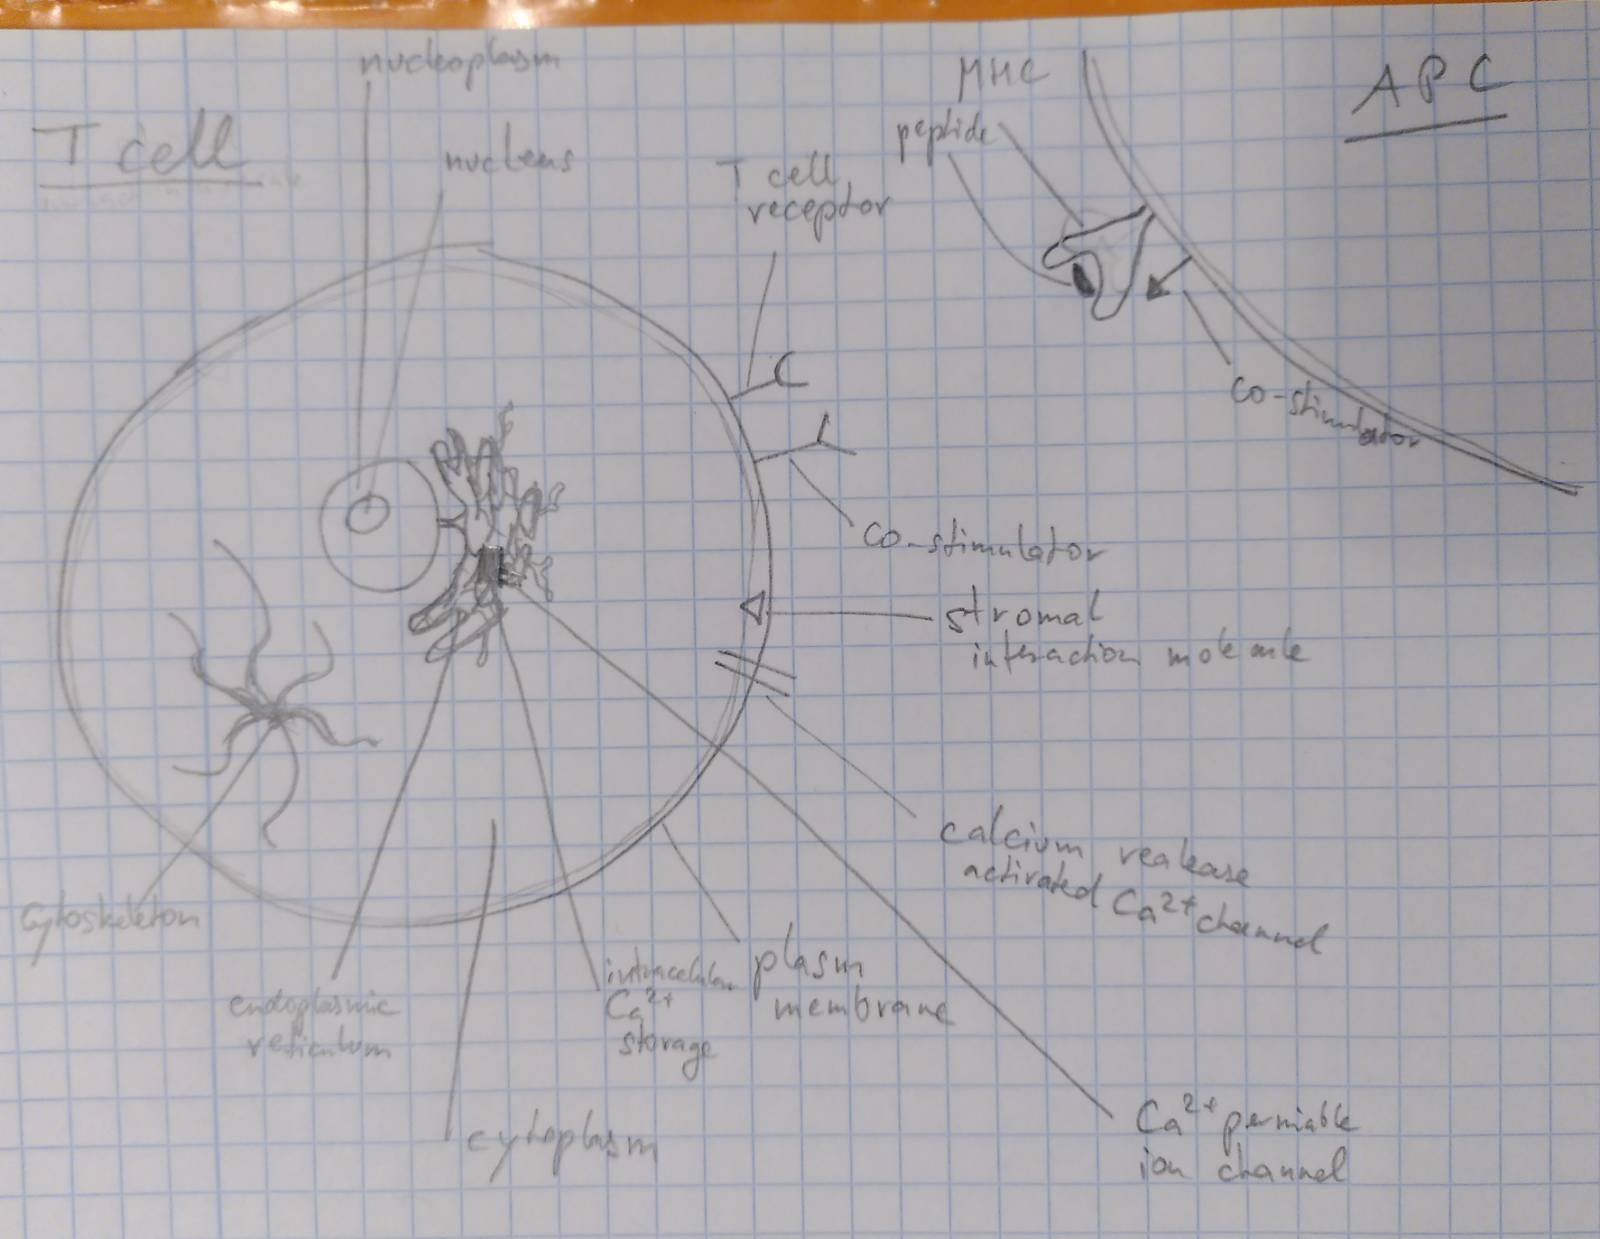
\includegraphics[width=\linewidth]{fig/tmp_t_cell_components}
	\caption{Schematic view of a t cell and antigen presenting cell, with all relevant components.}
	\label{fig:tcellcomponents}
\end{figure}

\section{Activation}
\label{sec:t-cell/activation}

Activation is necessary for t cells to divide and perform their functions.\cite{Ganong1997}

When a native t cell encounters a peptide on an APC that is compatible, a bond is formed between the TCR on the t cell and the peptide-MHC complex on the APC. This recognition can be triggered by less than ten molecules of foreign substance and is therefore described as near perfect. Sufficiently long contact is necessary between the APC and the t cell in order for the t cell to activate. The role of contact time in t cell activation is modelled by Morgan et al..\cite{morgan2023}.

The presence of co-stimulatory molecules is needed for proper activation. The bond between the co-stimulatory molecules on the t cell and APC plays a role in signalling. \Calcium signals play a vital part in t cell activation.

An increase of \Calcium in t cells during activation is caused by the stimulation of \Calcium permeable ion channel receptors on the ER membrane. \Calcium is released from the ER into the cytoplasm. Additionally, this decrease in \Calcium is sensed by STIM, which leads to an influx of \Calcium through plasma membrane CRAC channels.\cite{smith2009}

As the intracellular \Calcium concentration is dependent on the interaction between \Calcium sources and sinks, a variety of different forms in \Calcium concentration have been observed. Examples are infrequent spikes, sustained oscillations and plateaus.\cite{Lewis2001}

Intercellular \Calcium increase together with other signals lead to a redistribution of receptors, signalling molecules and organelles.\cite{joseph2014}
\chapter{Calcium Data of T Cells}
\label{chapter:data}

From section~\ref{sec:t-cell/activation}, we gather that analysing the intracellular \Calcium concentration gives us good insight in whether and when a cell activates. Additionally, it can be measured relatively easily by the method described in this chapter.

\section{Structure of the Data}
\label{sec:structure_of_data}

First we describe the structure of the data this work uses. 

The data matrix has one row for each tracked particle and frame combination. In this context cells are called particles as the recording might feature non-cells that are detected as a cell and recorded in the data set. The information stored for each particle and frame combination is described in detail in table~\ref{tab:information_data_matrix}.

\begin{table}[h!]
	\centering
	\begin{tabular}{|c|c|l|}
		\hline
		\textbf{Name} & \textbf{Data Type} & \textbf{Description} \\
		\hline
		x & float64 & Position of particle in pixels along the horizontal axis \\
		\hline
		y & float64 & Position of particle in pixels along the vertical axis \\
		\hline
		frame & int32 & Number of frame, with frame rate of 1 frame per second \\
		\hline
		mass short & float64 & Brightness of cell in 340nm channel \\
		\hline
		bg short & float64 & Background in 340nm channel \\
		\hline
		mass long & float64 & Brightness of cell in 380nm channel \\
		\hline
		bg long & float64 & Background in 380nm channel \\
		\hline
		ratio & float64 & Calculated as mass short divided by mass long \\
		\hline
		particle & int32 & Identification for each particle \\
		\hline
	\end{tabular}
	\caption{Description and data type of all columns present in the data matrix.}
	\label{tab:information_data_matrix}
\end{table}

% mouse pos: 4289, 720; mouse neg: 7683, 785; human pos: 694, 948

One recording can have between 500 and 10000 particles and is between 700 and 1000 frames long, which corresponds to between about 11 and 17 minutes. The ratio recorded is typically between 0 and 5.

Four recordings where generated, with two each from human and mouse cells. For each cell type a positive and negative control was measured. In a positive control the conditions are such, that in theory every cell should activate, while in negative control the conditions are such, that none should activate. Due to stress on the cells caused by the movement or changes in temperature and other factors a few cells will activate before the recording starts, during the recording in the negative control or not activate at all in the positive control, regardless of the conditions.

\section{Jurkat Cells, 5c.c7 Primary Mouse T Cells and Fura-2}

The prototypical cell line to study T cell signalling is the Jurkat cell line.\cite{morgan2023} It was obtained from the blood of a boy with T cell leukaemia.\cite{schneider1977} Different cell lines within the Jurkat family are described by Abraham and Weiss.\cite{abraham2004} They provide a timeline of discoveries linked to Jurkat cells and t cell receptor signalling.

Another type of T cells used in signalling studies are gathered from mice. [Additional information]

In order to be able to measure the intracellular \Calcium concentration of cells they can be labelled with Fura-2. This method provides a way to record the \Calcium concentration of multiple cells over a time period.\cite{martinez2017} Challenges encountered when using Fura-2 on certain cell types are described by Roe, Lemasters and Herman along with their respective solutions.\cite{roe1990}

\section{Measuring the Calcium Concentration of T Cells}

After the cells have been labelled with Fura-2, a recording of up to 15 to 20 minute can be generated. To achieve this the cells and stimulant are photographed at both 340nm and 380nm wavelength once per second. The resolution of the images are 1.6um per pixel. By calculating the ratio of the two images at each pixel the \Calcium concentration can be observed. An exemplary resulting image showing the ratio is shown in figure~\ref{fig:example_ratio_img}. The T cells appear a lighter shade than the background when activated and darker when not activated.

\begin{figure}
	\centering
	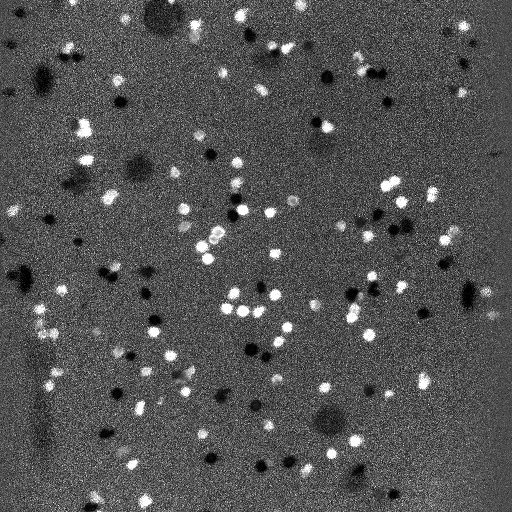
\includegraphics[width=0.6\linewidth]{fig/frame_ratio.jpg}
	\caption{Single frame showing the ratio of the 340nm and 380nm images from a recording of human Jurkat cells. Activated cells appear lighter, unactivated cells darker than the background. Big dark circles are out of focus cells that have not yet settled on to the plate.}
	\label{fig:example_ratio_img}
\end{figure}

To activate the cells in the duration of the recording they are transferred to a plate covered with replicas of the MHC-peptide complex normally present on APCs. This plate is then recorded as described above. For a negative control the plate is not covered with peptides, while for the positive control the peptide covering on the plate is very dense. Recordings of different densities in peptides lead to activation of a percentage of t cells.

\section{Processing the Data}

To track single t cells moving around during the video the sum of the 340nm and 380nm image of each second is calculated. This image provides the basis for separating t cells from the background. On this image all t cells will appear similarly light in colour. Therefore, it is used to track the movement of cells. Each cell is numbered, such that the same cell will have the same number during the video. For some cells the trajectory tracking is not perfect, resulting in a split of the numbering into multiple numbers for the same cell. The position and shade during both 340nm and 380nm as well as the ratio of each particle and each frame is then recorded into the data structure used in this work. The first roughly 50 frames at the start of the recording are discarded due to the video being out of focus. Additionally, cells only appearing in fewer than 300 frames are discarded as they most likely represent trajectories incorrectly tracked or split. The resulting data is then stored in a matrix structured as described in table~\ref{tab:information_data_matrix}.

\chapter{Modelling the Approximation of Calcium Concentration}
\label{chapter:approximating}

If we have a look at the typical trajectory of the calcium concentration in activated and unactivated cells, shown in figure~\ref{fig:all_cells_overlayed}, we can see differences emerging. For one, the maximum concentration value reached by most activated cells is higher. Another distinguishing feature is the presence of a steep incline at the moment of activation.

\begin{figure}[h]
	\centering
	\begin{subfigure}{0.45\linewidth}
		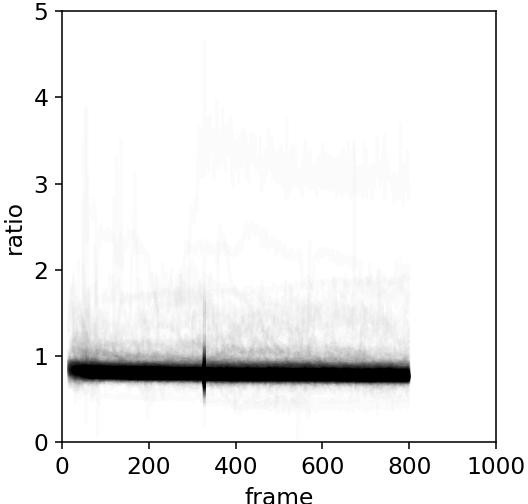
\includegraphics[width=\textwidth]{fig/all_cells_overlayed_mouse_neg}
	\end{subfigure}
	\hfill
	\begin{subfigure}{0.45\linewidth}
		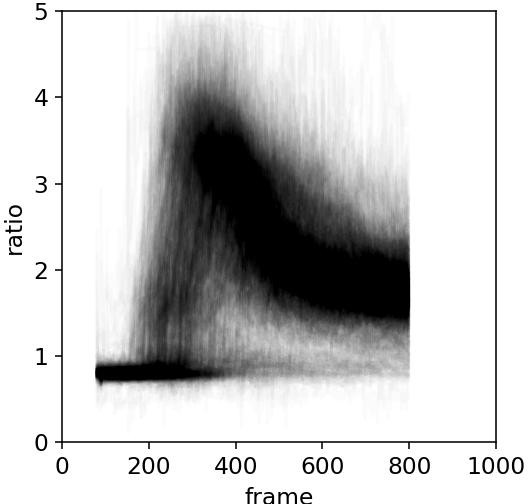
\includegraphics[width=\textwidth]{fig/all_cells_overlayed_mouse_pos}
	\end{subfigure}
	
	\caption{Two plots of the overlapping calcium concentration time series of cells, on the left a negative control and on the right a positive control of mouse cells.
	It is assumed that most cells from the negative control did not activate, while most of the cells from the positive control did.
	}
	\label{fig:all_cells_overlayed}
\end{figure}

By modelling the time series with a function incorporating features such as the increase, maximum value and oscillations present in the decrease afterwards, we can extract these features more easily. By doing this, using approximation methods from chapter~\ref{chapter:optimization}, we hope to have an easier method to answer the questions from the introduction.

\newpage
\section{Approximation Function}

From studying the data in the two control groups we find to expect a function close to
\begin{align}
	\label{math:function_unactivated_cell}
	f_{\text{unac}}(x) := u \in \mathds{R}
\end{align}
for unactivated cells and
\begin{align}
	\label{math:function_activated_cell}
	f_{\text{ac}}(x) := \begin{cases}
		\frac{a-u}{1 + \text{e}^{-k_1(x-w_1)}} + u & \textbf{ if } x <= t\\
		\frac{a-d}{1 + \text{e}^{-k_2(x-w_2)}} + d & \textbf{ else}
	\end{cases}
\end{align}
for activated cells. The parameters are described in table~\ref{tab:parameters}.

\begin{table}[h!]
	\centering
	\begin{tabular}{|c|l|}
		\hline
		\textbf{Variable} & \textbf{Description}\\
		\hline
		\hline
		$u$ & average value before activation\\
		\hline
		$a$ & value reached at the peak of activation\\
		\hline
		$d$ & average value after activation\\
		\hline
		$k_1$ & steepness of increase\\
		\hline
		$k_2$ & steepness of decrease\\
		\hline
		$w_1$ & time point at which the increase happens\\
		\hline
		$w_2$ & time point at which the decrease happens\\
		\hline
		$t$ & time point at which the increase ends, and the decrease starts\\
		\hline
	\end{tabular}
	\caption{List of parameters occurring in function $f_{\text{unac}}$ from~\ref{math:function_unactivated_cell} and function $f_{\text{ac}}$ from~\ref{math:function_activated_cell} and their interpretation.}
	\label{tab:parameters}
\end{table}

Figure~\ref{fig:typical_time_series_with_parameters} depicts the above functions~(\ref{math:function_unactivated_cell}), (\ref{math:function_activated_cell}), and the relations to the parameters in unactivated and activated cells. The similarity between these functions and figure~\ref{fig:all_cells_overlayed} can be observed.

% start = 50, u = 0.9, a = 4, k1 = 0.075, k2 = -0.04, w1 = 300, w2 = 520, t = 400, d = 2, z = 800

\begin{figure}[h!]
	\centering
	\begin{subfigure}{0.45\linewidth}
	  \begin{tikzpicture}
		\datavisualization [scientific axes, visualize as line,
			x axis = {
				min value = 0,
				max value = 1000,
				length = 5cm,
				ticks and grid = {major={at={0 as $t$}}, color=white},
				label = frame
			},
			y axis = {
				min value = 0,
				max value = 5,
				length = 5cm,
				ticks and grid = {major={at={0.9 as $u$}}},
				label = ratio
			},
		]
		data [format=function] {
			var x : interval [50:800]; func y = 0.9;
		};
	\end{tikzpicture}
	\end{subfigure}
	\hfill
	\begin{subfigure}{0.45\linewidth}
		\begin{tikzpicture}
			\datavisualization [scientific axes, visualize as line,
			x axis = {
				min value = 0,
				max value = 1000,
				length = 5cm,
				ticks and grid = {major={at={300 as $w_1$, 400 as $t$, 520 as $w_2$}}},
				label = frame
			}, y axis = {
				min value = 0,
				max value = 5,
				length = 5cm,
				ticks and grid = {major={at={0.9 as $u$, 2 as $d$, 4 as $a$}}},
				label = ratio
			},
			]
			data [separator=\space] {
				x y
				50 0.9000000223018123
				60 0.9000000472129365
				70 0.9000000999497857
				80 0.9000002115936903
				90 0.9000004479438116
				100 0.9000009482969035
				110 0.9000020075438745
				120 0.9000042499673413
				130 0.9000089971671542
				140 0.9000190469412669
				150 0.9000403220982461
				160 0.9000853606424553
				170 0.9001807029235496
				180 0.9003825231855573
				190 0.9008096899891967
				200 0.9017136137744631
				210 0.9036254818216721
				220 0.9076651317855678
				230 0.9161823896500311
				240 0.9340595221548389
				250 0.9712298467210794
				260 1.047020206850457
				270 1.1955833411872394
				280 1.4655191237997047
				290 1.8945460325562817
				300 2.45
				310 3.005453967443718
				320 3.434480876200295
				330 3.704416658812761
				340 3.8529797931495433
				350 3.9287701532789203
				360 3.9659404778451615
				370 3.983817610349969
				380 3.9923348682144324
				390 3.9963745181783277
				400 3.998286386225537
				410 3.9757431300314514
				420 3.964027580075817
				430 3.946806012846268
				440 3.9216685544064713
				450 3.8853516482022625
				460 3.8336546070121553
				470 3.7615941559557644
				480 3.664036770267849
				490 3.537049566998035
				500 3.379948962255225
				510 3.197375320224904
				520 3.0
				530 2.802624679775096
				540 2.620051037744775
				550 2.4629504330019647
				560 2.335963229732151
				570 2.238405844044235
				580 2.1663453929878447
				590 2.1146483517977375
				600 2.0783314455935287
				610 2.053193987153732
				620 2.035972419924183
				630 2.0242568699685486
				640 2.0163251423063198
				650 2.010972597798901
				660 2.007368479798872
				670 2.0049452463132695
				680 2.0033176021603487
				690 2.0022250720657206
				700 2.0014920576676736
				710 2.001000402214159
				720 2.0006707002609327
				730 2.0004496335404665
				740 2.0003014207161196
				750 2.0002020583878157
				760 2.0001354482992397
				770 2.000090795737405
				780 2.0000608631138013
				790 2.00004079817456
			}
			info {
			\draw (visualization cs: x=300, y=2.5)
			node [left,font=\footnotesize] {$k_1$};
			\draw (visualization cs: x=520, y=3.1)
			node [right,font=\footnotesize] {$k_2$};
			};
		\end{tikzpicture}
	\end{subfigure}
	
	\caption{Left shows the function $f_{\text{unac}}$ defined in~(\ref{math:function_unactivated_cell}) with the parameter $u$. The right shows the function $f_{\text{ac}}$ defined in~(\ref{math:function_activated_cell}) with the parameters $u$, $d$, $a$, $w_1$, $t$, $w_2$, $k_1$ and $k_2$.}
	\label{fig:typical_time_series_with_parameters}
\end{figure}

For our model to make sense, we have to impose some conditions on the parameters. We expect
\begin{align}
	\label{eq:conditions}
	0 \leq u \leq d \leq a, && w_1 \leq t \leq w_2, && k_1 > 0 && \text{and} && k_2 < 0.
\end{align}

There are multiple ways in which the parameters of $f_{\text{ac}}$ can be chosen to get a function similar to $f_{\text{unac}}$. If $w_1$ is very large or $u \approx d \approx a$ then $f_{\text{ac}}$ approaches a constant value of $u$, thus approximating $f_{\text{unac}}$. If the approximation of a cell has parameters with $w_1$ very large or $u \approx d \approx a$ we can therefore expect it to be of an unactivated cell. Otherwise, it is more probable to be activated.

\newpage
\section{Implementation of the Approximation Model}

Now that we have defined our model functions we will implement a routine that fits such a $f_{\text{ac}}$-function through the data points of a particle recording.

First we give the pseudocode for approximating a single particles time series with the approximation function described above. It takes a (frame, ratio)-matrix of a single particle as input and returns the corresponding parameter list of the approximation.

\begin{algorithm}[H] \label{alg:approximate}
	\SetAlgoLined
	\DontPrintSemicolon
	\LinesNumbered
	\SetKwInOut{Input}{input}
	\SetKwInOut{Output}{output}
	\caption{Approximation of the Calcium Concentration}
	
	\Input{particle data as (frame, ratio)-matrix}
	\Output{parameters describing the approximation}
	
	\BlankLine
	\Begin{
		set boundaries for parameters\;
		set start values for parameters\;
		use Trust Region Reflective Algorithm with boundaries and start values to get parameters\;
		calculate corresponding approximation and add as fit\_sigmoid columns to data matrix\;
		\Return{parameters}\;
	}
\end{algorithm}

The parameters of $f_{\text{ac}}$ used in the approximation are not independent of each other as we want to choose $t$ to be the point at which the increasing part of the function, ${(a-u)/(1+\text{e}^{-k_1(x-w_1)})}$, almost reaches the value $a$. We choose
\begin{align*}
	t := w_1 - \frac{\log_e\left(\frac{1}{0.99}-1\right)}{k_1} = w_1 - \frac{1}{k_1} \log_e\left(\frac{1}{99}\right),
\end{align*}
as the function has had $99\%$ of the increase of the sigmoid curve up to this point.

Setting the boundaries in line 2 is non-trivial. We have noted that the conditions from equation~\ref{eq:conditions} are expected. We want to impose them using boundaries in which the parameters must lie. However, boundaries for each parameter must not depend on other parameters. We can circumvent this by changing the parameters to be relative to each other. As $u \leq d \leq a$ we choose to use the three parameters $u, d-u$ and $a-d$. Then, we can set the lower boundary to be $0$ which ensures
\begin{align*}
	0 \leq u &&\land &&0 \leq d - u \implies d \geq u &&\land &&0 \leq a - d \implies a \geq d\\
	&& &&\implies 0 \leq u \leq d \leq a.
\end{align*}

Using the same method, we choose the parameters $w_1 - start$ and $w_2 - w_1$, where $start$ is the first frame in which the particle was tracked. The resulting boundaries are described in table~\ref{tab:boundaries_and_starting_vals}, where we set min val, max val and median val as the minimum, maximum and median of the particles' ratio data respectively while start and end is the first and last frame where data was recorded for this particle.

The condition $t \leq w_2$ can be violated, but it is ensured that at least $w_1 \leq w_2$. The other conditions are met as $k_1 \in [0.05, 10] \implies k_1 > 0$ while $k_2 \in [-1, -0.01] \implies k_2 < 0$ and
\begin{align*}
	t = w_1 - \underbrace{\frac{1}{k_1} \log(\frac{1}{99})}_{< 0} \geq w_1.
\end{align*}

Along with the boundaries we specify so-called starting values. These define to which values the parameters are set at the start of the approximation algorithm.

\begin{table}[h!]
	\centering
	\begin{tabular}{|c|c|c|c|}
		\hline
		\textbf{parameter} & \textbf{lower bound} & \textbf{upper bound} & \textbf{starting value} \\ 
		\hline
		\hline
		$u$ & min val & max val & min val\\
		\hline
		$d - u$ & 0 & max val & median val - min val\\
		\hline
		$a - d$ & 0 & max val & max val - median val\\
		\hline
		$w_1 - start$ & 0 & end - start & 0\\
		\hline
		$w_2 - w_1$ & 0 & end - start & (end - start) / 2\\
		\hline
		$k_1$ & 0.05 & 10 & 0.1\\
		\hline
		$k_2$ & -1 & -0.01 & -0.03\\
		\hline
		\hline
		$d$ & min val & 2 max val & median val \\
		\hline
		$a$ & min val & 3 max val & max val \\
		\hline
		$w_1$ & start & end & start \\
		\hline
		$w_2$ & start & 2 end - 2 start & (start + end)/2\\
		\hline
	\end{tabular}
	\caption{Upper and lower bounds as well as starting value for each of the parameters. The boundaries and starting values of $d, a, w_1$ and $w_2$ are derived from the parameters used in the implementation of the approximation, shown above the double line.}
	\label{tab:boundaries_and_starting_vals}
\end{table}

Starting values can have a big impact on the approximation reached by the algorithm. We want to choose starting values close to the expected resulting parameters. By choosing the starting value of $w_1 - start$ as $0$, which corresponds to choosing $w_1 = start$, we favour the first increase in the data to be the point of activation. Otherwise, we are more likely to mistake an oscillation later in the data as the activation point. As we do not know when the activation happens when setting the boundaries we guess that $w_2$ will lie somewhere in the middle. Therefore we choose $(end - start)/2$ as the starting value for $w_2 - w_1$. The other starting values are chosen as we expect $u$ to be low, $a$ to be high, $d$ to lie somewhere in the middle. Experimenting showed that $k_1$ often has a value around $0.1$ while $k_2$ lies around $-0.03$.

Using algorithm~\ref{alg:approximate} we now describe a routine which handles reading the data, some necessary preprocessing steps and saving of the resulting parameter lists.

\begin{algorithm}[H] \label{alg:main}
	\SetAlgoLined
	\DontPrintSemicolon
	\LinesNumbered
	\SetKwInOut{Input}{input}
	\SetKwInOut{Output}{output}
	\caption{Approximation Loop}
	
	\Input{file containing data matrix as described in section \ref{sec:structure_of_data}}
	\Output{parameters of the approximation of all particles as a matrix}
	
	\BlankLine
	\Begin{
		read data\;
		filter data\;
		\For{each single particle}{
			particle data := (frame, ratio) columns of this particle\;
			\If{length of particle data is too short}{
				skip\;
			}
			parameters := approximate(particle data)\;
			optionally show ratio data and approximation\;
			save parameters\;
		}
		\Return{matrix of all parameters}
	}
\end{algorithm}
\vspace{1cm}

Filtering the data is necessary as the ratio can be very large if the denominator is small. Values are therefore bounded to lie within the interval $[0, 5]$. Any values higher than 5 are almost certainly caused by measurement errors. Values below 0 are definitely incorrect, as both the denominator and enumerator are measured as the brightness of a pixel, which can not be negative.

The visualization in line 10 of algorithm~\ref{alg:main} generates images such as figure~\ref{fig:particle_vis_sigmoid_approx}. It depicts the approximation of two T cells, one of which is activated during the recording, while the other is not. The ratio data recorded is shown in black, while the approximation is shown in orange. It is important to note that the approximation performed on unactivated T cells still uses the same function $f_{\text{ac}}$.

\begin{figure}[h]
	\centering
	\begin{subfigure}{0.48\linewidth}
		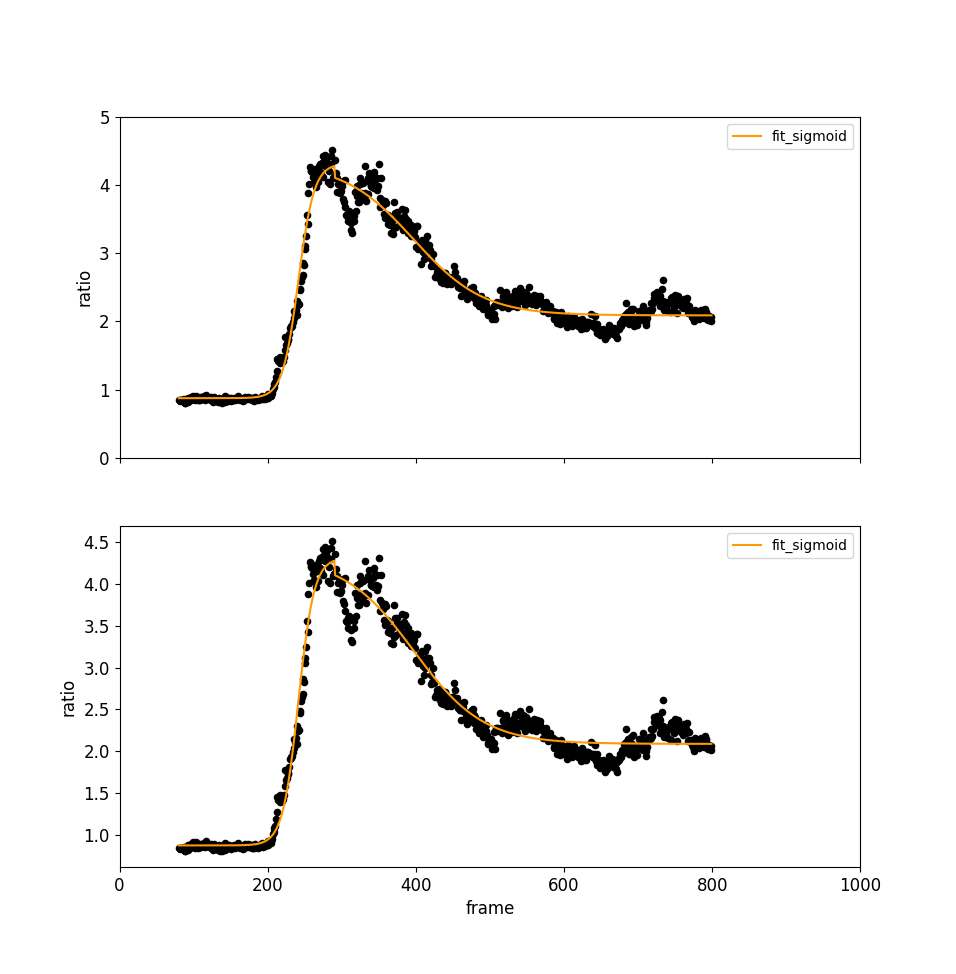
\includegraphics[width=\textwidth]{fig/particle_vis_sigmoid_approx_pos}
	\end{subfigure}
	\hfill
	\begin{subfigure}{0.48\linewidth}
		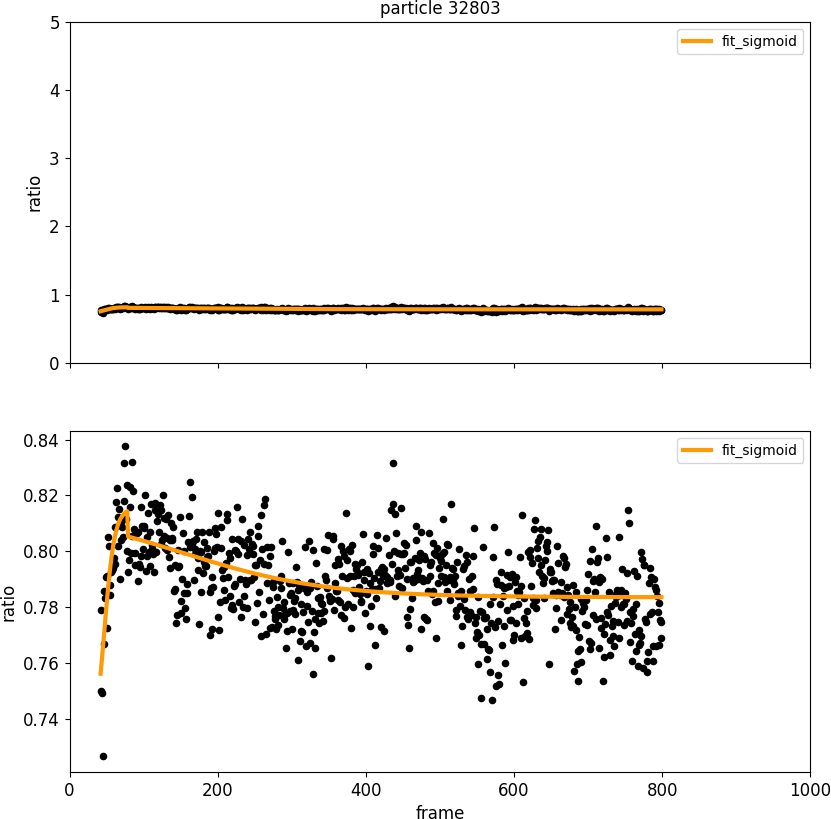
\includegraphics[width=\textwidth]{fig/particle_vis_sigmoid_approx_neg}
	\end{subfigure}
	
	\caption{The left plot shows the data in black and approximation in orange of an activated cell. The upper plot is scaled from 0 to 5, the lower one is scaled to fit the data. The right plot shows the same of an unactivated cell.}
	\label{fig:particle_vis_sigmoid_approx}
\end{figure}

This work uses the python scipy function \texttt{scipy.optimize.curve\_fit(function,\\ xdata, ydata, p0=starting\_values, method='trf', bounds=(lower\_bounds,\\ upper\_bounds))} as it provides all the necessary functionality. The method parameter \texttt{trf} stands for Trust Region Reflective, as described in section~\ref{subsec:algorithms_bounded_lsp}.

\section{Analysis of the Approximation}
\label{sec:analysis_of_approximation}

We now give detailed information on the parameters found from the above approximation. Some statistics are found in table~\ref{tab:statistics_parameters}.

\begin{table}[h!]
	\centering
	\begin{tabular}{|c|c|c|c|c|c|c|}
		\hline
		& & \multicolumn{2}{c|}{\textbf{Positive Control}} & \multicolumn{2}{c|}{\textbf{Negative Control}} & \\ 
		\hline
		& \textbf{Parameter} & $\mu$ & $\sigma$ & $\mu$ & $\sigma$ & \textbf{Difference} \\ 
		\hline
		\hline
		\multirow{7}{*}{\rotatebox[origin=c]{90}{\textbf{human cells}}} & $a$ & 2.808 & 0.461 & 0.923 & 0.669 & 1.885\\
		\cline{2-7}
		& $u$ & 0.663 & 0.521 & 0.613 & 0.311 & 0.05\\
		\cline{2-7}
		& $d$ & 1.937 & 0.491 & 0.685 & 0.412 & 1.252\\
		\cline{2-7}
		& $k_1$ & 0.263 & 0.428 & 0.524 & 0.963 & -0.261 \\
		\cline{2-7}
		& $k_2$ & -0.059 & 0.164 & -0.163 & 0.292 & 0.104 \\
		\cline{2-7}
		& $w_1$ & 142.228 & 124.012 & 171.062 & 131.563 & -28.834 \\
		\cline{2-7}
		& $w_2$ & 445.386 & 185.971 & 478.843 & 190.792 & -33.457 \\
		\hline
		\hline
		\multirow{7}{*}{\rotatebox[origin=c]{90}{\textbf{mouse cells}}} & $a$ & 2.9 & 0.907 & 0.876 & 0.186 & 2.024 \\
		\cline{2-7}
		& $u$ & 0.889 & 0.27 & 0.79 & 0.093 & 0.099 \\
		\cline{2-7}
		& $d$ & 1.749 & 0.407 & 0.804 & 0.129 & 0.945 \\
		\cline{2-7}
		& $k_1$ & 0.15 & 0.409 & 1.161 & 1.235 & -1.011 \\
		\cline{2-7}
		& $k_2$ & -0.1 & 0.195 & -0.133 & 0.267 & 0.033 \\
		\cline{2-7}
		& $w_1$ & 295.809 & 77.207 & 100.712 & 112.352 & 195.097 \\
		\cline{2-7}
		& $w_2$ & 469.952 & 105.375 & 304.283 & 179.834 & 165.669 \\
		\hline
	\end{tabular}
	\caption{Average $\mu$ and standard deviation $\sigma$ of the parameters retrieved from approximating the human cell data.}
	\label{tab:statistics_parameters}
\end{table}

Figure~\ref{fig:parameter_violin_plot} shows the distribution of the resulting parameters of the approximation. From the figure it seems the differences between activated and unactivated cells is biggest in the parameters activated value $a$, decreased value $d$ as well as the steepness of increase $k_1$.

\begin{figure}[h!]
	\centering
	\begin{subfigure}{0.45\linewidth}
		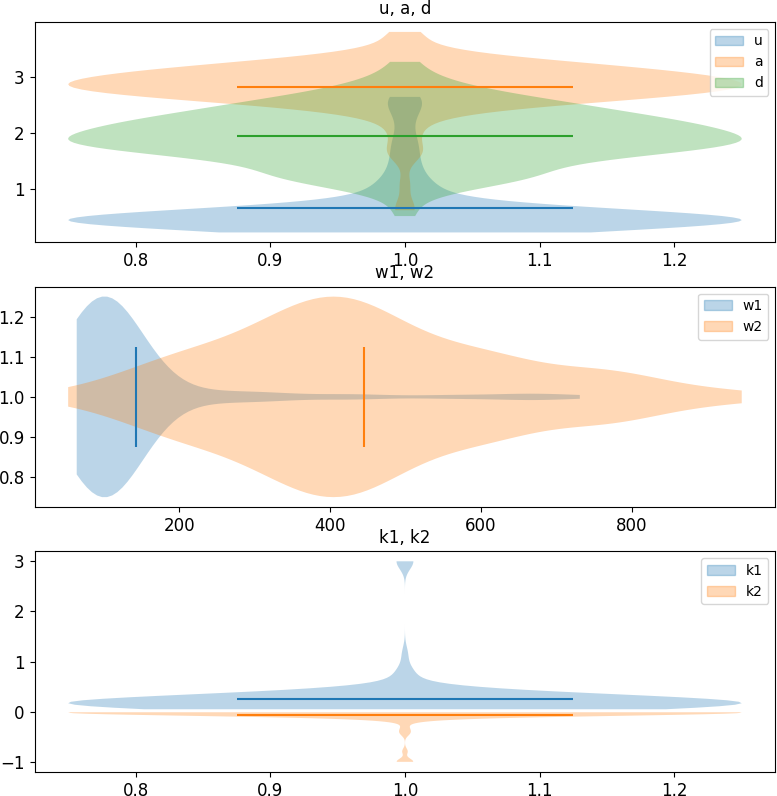
\includegraphics[width=\textwidth]{fig/parameter_violin_plot_human_pos}
	\end{subfigure}
	\hfill
	\begin{subfigure}{0.45\linewidth}
		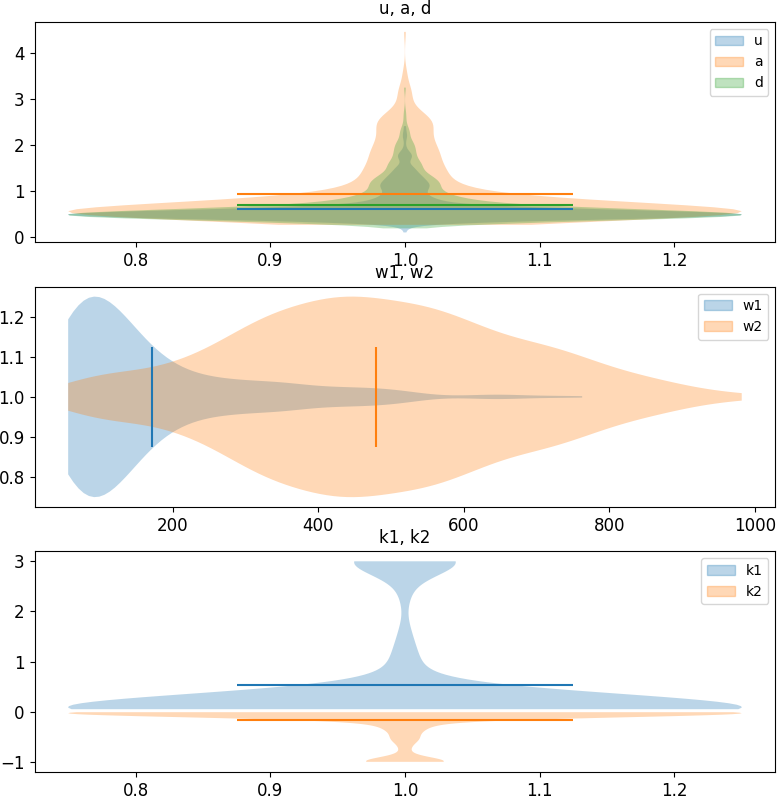
\includegraphics[width=\textwidth]{fig/parameter_violin_plot_human_neg}
	\end{subfigure}
	
	\caption{Violin plots of parameters $u, a, d, w_1, w_2, k_1$ and $k_2$ from the approximations. The mean is shown by the bar. The width of the individual plots corresponds to the distribution density. The parameters of the positive control are on the left and those of the negative control are on the right. Both are of human cells.}
	\label{fig:parameter_violin_plot}
\end{figure}

As the datasets are not perfectly labelled, meaning there are activated cells in the negative control and vice versa, we have relatively high standard deviation.

We can use the mean and standard deviation of each of the parameters to find data points that can be considered outliers. We expect wrongly-labelled data, e.g. activated cells in the negative control, to be an outlier in the parameters $a$ and $d$. However, activated cells in the positive control might have a decreased value $d$ that is very low, around $u$. This makes it difficult to distinguish activated from unactivated cells when looking at the parameter $d$. Therefore, we choose $a$ as the only parameter when filtering for these kinds of outliers.

A particle from the positive control dataset that has a value in parameter $a$ higher than the median should still be classified as activated. Only a value lower than some threshold indicates an unactivated cell. The same holds for values of $a$ lower than the median in the negative control dataset. In short, we want to filter out particles with a high value of $a$ in the negative control and those with a low value of $a$ in the positive control dataset. Therefore, the threshold has to be specified as a lower and upper bound in multiples of the standard deviation.

We give pseudocode for the detection of outliers in algorithm~\ref{alg:outlier_detection}.
\newpage

\begin{algorithm}[H] \label{alg:outlier_detection}
	\SetAlgoLined
	\DontPrintSemicolon
	\LinesNumbered
	\SetKwInOut{Input}{input}
	\SetKwInOut{Output}{output}
	\caption{Find Outliers}
	
	\Input{data as matrix of all particle parameters of the approximation, threshold as pair, parameters\_used as list}
	\Output{set of indices of the outliers}
	
	\BlankLine
	\Begin{
		outliers := empty set\;
		\For{parameter in parameteres\_used}{
			mean := mean(data[parameter])\;
			std := standard\_deviation(data[parameter])\;
			interval := [mean - std $\cdot$ threshold[0], mean - std $\cdot$ threshold[1]]\;
			outliers = outliers $\cup$ \{data[index] : data[parameter] $\not\in$ interval\}\;
		}
		\Return{outliers}
	}
\end{algorithm}
\vspace{1cm}

The question of how to choose the threshold will be discussed next. As we do not have information on what percentage of cells behaved correctly in the positive and negative control we do not have enough information to choose threshold values without guessing. Instead, we can manipulate the threshold as a multiple of the standard deviation until we filter out incorrectly labelled data, but would filter out correctly labelled data points if we increase the value. This trial and error approach led to different values for each of the four control datasets, which can be seen in table~\ref{tab:threshold_outlier}.

\begin{table}[h!]
	\centering
	\begin{tabular}{|c|c|c|}
		\hline
		\textbf{dataset} & \textbf{lower bound} & \textbf{upper bound}\\
		\hline
		\hline
		human positive & mean $ - 3$ std $ = 1.582$ & $\infty$ \\
		\hline
		human negative & $-\infty$ & mean $ + 0.5$ std $ = 1.306$ \\
		\hline
		mouse positive & mean $ - 2$ std $ = 1.41$ & $\infty$ \\
		\hline
		mouse negative & $-\infty$ & mean $ + 3$ std $ = 1.445$ \\
		\hline
	\end{tabular}
	\caption{Thresholds in outlier detection in the different datasets.}
	\label{tab:threshold_outlier}
\end{table}

Naturally we can use the same outlier detection with different parameters to find particles where the approximation failed to yield a good result.

These results will be used in section~\ref{sec:proposed-algorithm} to remove wrongly-labelled data from the datasets.

\section{Adding Oscillation to the Approximation}
\label{sec:adding_oscillation_to_the_approximation}

In order to answer the questions from chapter~\ref{chapter:introduction} concerned with the oscillations  happening in the decrease of the \Calcium concentration we want to model them as well. We use a method often used when analysing oscillating data, called Fourier Transformation.

Fourier Transformation is used when an application is concerned with cyclic temporal data. Examples are sound waves, seismic data or oscillations of a skyscraper in strong wind. This data can be represented as a function of amplitude over time. Most of the time we are not interested in the amplitude at a specific point in time, as a temporal shift would represent very similar information.
% Such a shift is demonstrated in figure~\ref{fig:tempoal_shift}.

%\begin{figure}[h]
%	\centering
%	
%	\begin{subfigure}[b]{\textwidth}
%		\begin{tikzpicture}
%			\begin{axis}[xlabel=Time, ylabel=Amplitude, width=\textwidth, height=0.4\textwidth]
%				\addplot+ [domain=0:pi, samples=100, no marks, color=black, style=solid]{0};
%				\addplot+ [domain=pi:3*pi, samples=100, no marks, color=black, style=solid]{sin(deg(x)) + 0.5*sin(deg(4*x)) + 0.1*sin(deg(10*x))};
%				\addplot+ [domain=3*pi:15, samples=100, no marks, color=black, style=solid]{0};
%				
%				\addplot+ [domain=0:pi+2, samples=100, no marks, color=red, style=solid]{0};
%				\addplot+ [domain=pi+2:3*pi+2, samples=100, no marks, color=red, style=solid]{sin(deg(x-2)) + 0.5*sin(deg(4*(x-2))) + 0.1*sin(deg(10*(x-2)))};section
%				\addplot+ [domain=3*pi+2:15, samples=100, no marks, color=red, style=solid]{0};
%			\end{axis}
%		\end{tikzpicture}
%	\end{subfigure}
%	
%	\caption{Two signals that differ by a temporal shift.}
%	\label{fig:tempoal_shift}
%\end{figure}

As the function of oscillations in the \Calcium concentration in T cells is almost cyclic we might be interested in a decomposition into simple cyclic functions, such as sinoid functions. Then, we can analyse the most prominent frequencies and their respective amplitudes. This gives a representation of the data, that can be easier to interpret. Fast Fourier Transformation (FFT) is an algorithm that transforms temporal data into such a representation of a weighted sum of sines. Pseudocode and a detailed description are provided by Cormen et al\cite{Cormen2009}.

As the oscillations happen in the decrease of the \Calcium concentration we apply FFT to that part of the data. We can use the frequency with the highest amplitude and use them to further analyse the oscillations. After having found this estimation of the frequency we can use the method from before, but with a sine function instead of the sigmoid functions. In detail, we once again utilize \texttt{scipy.optimize.curve\_fit}, this time using the function
\begin{align*}
	f(x, A, \omega, p) := A \cdot \sin(\omega \cdot t + p),
\end{align*}
with parameters amplitude $A$, angular frequency $\omega$ and phase $p$. The starting value for the approximation can be set using the results of the FFT. We denote the frequency with the highest amplitude returned from the FFT by $freq_{guess}$ and the standard deviation of the approximation residuum time series with $std(Y)$. Then, we can set the start value of $A$ to be $\sqrt{2 \cdot std(Y)}$, the one of $\omega$ to be $2\pi |freq_{guess}|$ and the one of $p$ to be $0$.

The drawback of this method is that only oscillations that can be represented by a single sine function can be modelled. However, for our purpose we can assume that the oscillations are of this form.
This gives an even better approximation of the data, which can be seen in figure~\ref{fig:particle_vis_fft_approx}.

\begin{figure}[h]
	\centering
	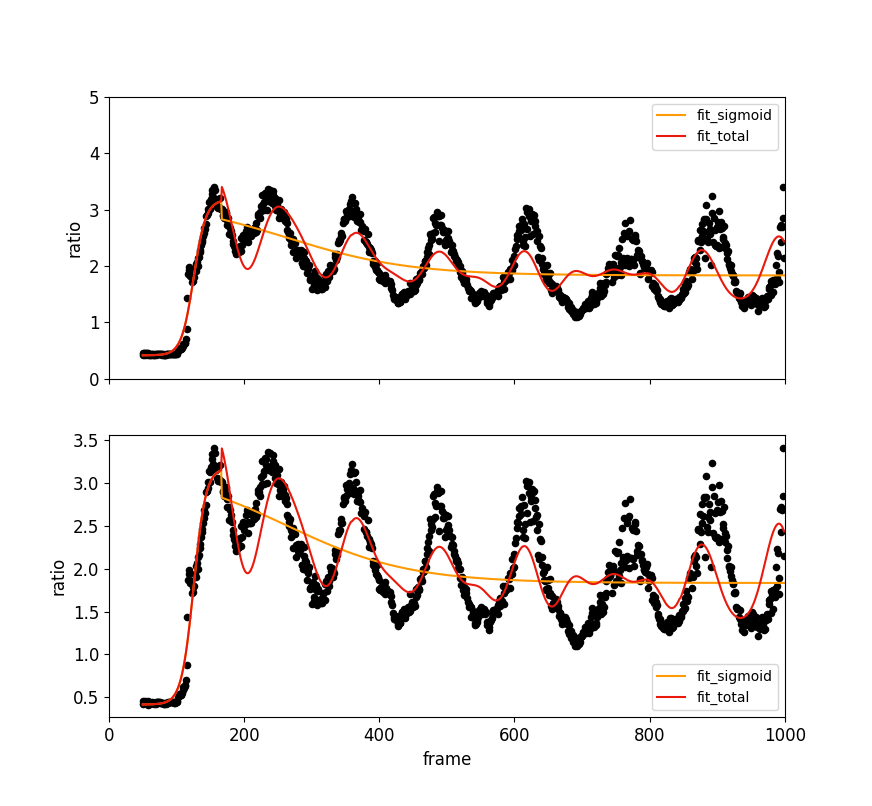
\includegraphics[width=0.9\textwidth]{fig/particle_vis_fft_approx_pos}
	
	\caption{The data of an activated cell with heavy oscillations is shown in black, simple approximation in orange and the approximation with FFT added in red. The first plot is scaled from 0 to 5, the second one is scaled to fit the data.}
	\label{fig:particle_vis_fft_approx}
\end{figure}

We store the data gathered from the approximation as a list of frequency, amplitude and phase.

\chapter{Clustering}

The objective of classification is to find assignments between data points and categories. For some applications this can be done by taking correctly labelled data and comparing a new data point to the data points in different categories to see which category best fits. One such algorithm is k-nearest-neighbour. In our context the issue with this approach is that the data is only labelled as to which experiment it came from, e.g. positive control in human cells, negative control in mouse cells. However, as noted before not all cells from these experiments behaved as we expected them to, e.g. some activated in the negative control or did not activate in the positive control. Therefore, we choose to use a clustering algorithm which does not have the need for classified training data.

\section{Gaussian Mixture Model}
\label{sec:gaussian_mixture_model}

This section follows the article Gaussian Mixture Model by Reynolds~\cite{reynolds2009}.

Often gathered observations are distributed as a normal distribution. These distributions have a density function
\begin{align*}
	g(x|\mu, \Sigma) = \frac{1}{(2\pi)^{D/2} |\Sigma|^{1/2}} exp\left( - \frac{1}{2} (x-\mu)^T \Sigma^{-1} (x-\mu) \right)
\end{align*}
with parameters $D$ as the dimension, $\mu$ as the mean vector and $\Sigma$ as the covariance matrix.

As we are concerned with clustering data we expect the observed data from different clusters to have different parameters in the normal distribution they come from. Assuming we have $n$ different data sources gives us normal distributions $g_i(x|\mu_i, \Sigma_i)$ where $i=1, ..., n$. Additionally, we might have more data points being generated from some normal distributions while less from others. We can express this using another weight parameter $w_i$ with $i=1, ..., n$. To normalize the weights we set the constraint $\sum w_i = 1$.

The distribution describing the entire dataset now can be described with the distribution
\begin{align}
	\label{eq:sum_of_normal}
	p(x) = \sum_{i=1}^{n} w_i g(x|\mu_i, \Sigma_i).
\end{align}

Gaussian Mixture Model is a method to retrieve these parameters $w_i$, $\mu_i$ and $\Sigma_i$ for some $D$ dimensional data points generated from $n$ normal distributions.

From these parameters it is easy to cluster the data as we know where data points from the different clusters are expected to lie.

From equation~\ref{eq:sum_of_normal} we expect every $\Sigma_i$ to be independent of each other. In the context of Gaussian Mixture Models this is called having a full covariance matrix. However, we can eliminate some of the variables in the covariance matrix if we choose a diagonal covariance matrix. Additionally, we might specify to use the same covariance matrix for all $i$, which is called tied in this context.

Choosing a full covariance matrix is not necessary even if the data is expected to have statistically independent features, as the overall density is compromised from multiple normal distributions with diagonal $\Sigma_i$. This enables us to model correlations between features.

The question now is how we can derive the parameters $w_i, \mu_i$ and $\Sigma_i$. We choose the approach which chooses the parameters where the likelihood that the data was generated by these parameters is maximal. This is known as maximum likelihood estimation. The likelihood can be expressed as

\begin{align*}
	L(w_i, \mu_i, \Sigma_i|X) = p(X|w_i, \mu_i, \Sigma_i) = \prod_{t=1}^n p(x_t|w_i, \mu_i, \Sigma_i)
\end{align*}

with $X = (x_1, ..., x_n)$ being the recorded data. As $L(w_i, \mu_i, \Sigma_i|X)$ is non-linear in the parameters deriving the maximum is not trivial. Instead, we use an iterative approach which approaches the solution. Define $\lambda = (w_i, \mu_i, \Sigma_i)$. Simplifying to a diagonal covariance matrix gives us the iterative algorithm where we define the successor values $\bar{.}$ as

\begin{align*}
	Pr(i | x_t, \lambda) := \frac{w_i g(x_t | \mu_i, \Sigma_i)}{\sum_{k=1}^{n} w_k g(x_t | \mu_k, \Sigma_k)}\\
	\bar{w}_i := \frac{1}{n} \sum_{t=1}^{n} Pr(i | x_t, \lambda)\\
	\bar{\mu}_i := \frac{\sum_{t=1}^{n} Pr(i | x_t, \lambda) x_t}{\sum_{t=1}^{n} Pr(i | x_t, \lambda)}\\
	\bar{\sigma}_i^2 := \frac{\sum_{t=1}^{n} Pr(i | x_t, \lambda) x_t^2}{\sum_{t=1}^{n} Pr(i | x_t, \lambda)} - \bar{\mu}_i^2.
\end{align*}

for $w_i$, $\mu_i$ and $\sigma_i^2$ respectively. One can show that with this iteration rule we have $p(X|\bar{\lambda}) \geq p(X|\lambda)$. The value $Pr(i|x_t, \lambda)$ is known as the a posteriori probability for the i-th component.

% https://scikit-learn.org/stable/modules/mixture.html#gmm

\section{Implementation}

Python offers an implementation of Gaussian Mixture Model with the sklearn package. The function with parameters relevant to us is \texttt{sklearn.mixture.GaussianMixture(n\_components, covariance\_type)}. The number of components \texttt{n\_components} can be any positive integer. The \texttt{covariance\_type} can be one of \texttt{‘full’, ‘tied’, ‘diag’} or \texttt{‘spherical’} and describes what type of covariance matrix is used.

As the input of the Gaussian Mixture Model we use data points of the form \texttt{[a, u, d, k1, k2, w1, w2]}, where \texttt{a, u, ..., w2} are the parameters of the approximation from chapter~\ref{chapter:approximating}. As our goal is to separate data points from the four data sets mouse cells and human cells each with a negative and a positive control, we use all particles as input. The pseudo code below describes the steps performed to reach a clustering of the data.

\begin{algorithm}[H] \label{alg:separate}
	\SetAlgoLined
	\DontPrintSemicolon
	\LinesNumbered
	\SetKwInOut{Input}{input}
	\SetKwInOut{Output}{output}
	\caption{Separate}
	
	\Input{approximation parameters of all particle data sets}
	\Output{assignments to different clusters}
	
	\BlankLine
	\Begin{
		initialize Gaussian Mixture by specifying \texttt{n\_components} and \texttt{covariance\_type}\;
		apply Gaussian Mixture to approximation parameters of all particle data sets\;
		assign particles to clusters according to Gaussian Mixture results\;
		compare asignments from Gaussian Mixture to those of the data set the data stems from\;
	}
\end{algorithm}
\vspace{1cm}

When comparing different covariance types in the Gaussian Mixture we see that using \texttt{‘diag’} we have the lowest error rate. The details are shown in table~\ref{tab:covariance_type_comparison}. Why reducing the number of parameters in the covariance matrix can yield better results is described in section~\ref{sec:gaussian_mixture_model}.

\begin{table}[h!]
	\centering
	\begin{tabular}{|c|c|}
		\hline
		\texttt{full}: $13.23\%$ & \texttt{tied}: $12.7\%$ \\
		\hline
		\texttt{diag}: $7.17\%$ & \texttt{spherical}: $31.52\%$ \\
		\hline
	\end{tabular}
	\label{tab:covariance_type_comparison}
	\caption{Error as a percentage of particles being assigned the wrong component.}
\end{table}

Using a diagonal covariance matrix we can now try to separate the four data sets and visualize the results. As the data is 7 dimensional we show lower dimensional representations of the data both as it is assigned according to the data set it stems from as well as the assignment from algorithm~\ref{alg:separate}.

[TODO visualization of seperation algorithm, choose good axis, maybe show multiple different axis, 2d]

The relevant information derived from the Gaussian Mixture clustering is the means and covariances of the four components. From this we can decide which cluster a new data point belongs to. A use case might be to find percentages of activated cells in an experiment. Distinguishing between mouse and human cells does not have a clear use case. When specifying \texttt{n\_components=2} we assume to have a cluster for activated and a second for unactivated cells.

The mean and covariances for each of the data sets used in this work are 

\begin{align*}
	\text{human positive}\\
	\text{human negative}
\end{align*}

\chapter{Results}
\label{chapter:results}

Combining all the methods and algorithms from the previous chapters, such as approximation, clustering and outlier detection, gives us insight into the \Calcium concentration data. We give an algorithm for detecting activated t cells, look at differences between mouse and human t cells, analyse the oscillations and investigate whether there are different types of activated t cells.

\section{Proposed Algorithm for Detecting Activated T Cells}
\label{sec:proposed-algorithm}

A relevant question this work aims to provide an answer to is how pre-activated, unactivated and activated t cells can be distinguished.

First we give a method for filtering the pre-activated cells from a dataset. From their nature we expect a high value in \Calcium concentration at the start of the recording. Using the approximation from chapter~\ref{chapter:approximating} it is easy to get the approximate \Calcium concentration value at the start of the recording, as it is the parameter $u$. Using the algorithm~\ref{alg:outlier_detection} with parameters threshold as $[\infty, 0.5]$ and parameters\_used as [$u$] gives good results. It returns the indices of particles, which are pre-activated in the data sets of the positive controls.

After having filtered out pre-activated particles, we want to distinguish between unactivated and activated particles. For this we propose the following steps:

\begin{enumerate}
	\item get positive control, negative control and experiment recordings
	\item transform each particle time series of all three data sets to the parameter list by approximating it with a combination of sigmoid functions, according to chapter~\ref{chapter:approximating}, using the algorithm \ref{alg:main}
	\item normalise each of the parameters of all data sets, such that the mean is 0 and the standard deviation is 1
	\item use outlier detection, which is described in algorithm~\ref{alg:outlier_detection}, to filter out non-conforming cells from both the positive and negative control, as well as pre-activated cells, and particles where the approximation yielded suboptimal results
	\item sample particles from the filtered positive and negative control groups to match the number of particles in the both groups
	\item use clustering method, as one of the two described in chapter~\ref{chapter:clustering}, with parameters of selected negative and positive control as input to get the clustering parameters
	\item predict the membership of the experiment particle parameters to the clusters to get a prediction of activation
\end{enumerate}

The third and fifth step is beneficial when clustering, as many clustering methods expect equally sized clusters that are centred and have equal standard deviation. 

This algorithm is implemented in Python and shown in appendix~\ref{chapter:python_implementation}. Applying this to a positive, negative control and an experiment data sets of mouse t cells gives the exemplary results shown in table~\ref{tab:results_main_algorithm}. The experiment dataset contains t cells that came in contact with a medium density of MHC-peptide complex replicas. The number of activated cells detected in the positive and negative control are shown as a reference point. Comparing them in the case illustrated suggests that in this case Gaussian Mixture Model is the better clustering algorithm.

\begin{table}[h]
	\centering
	\begin{tabular}{|c|c|c|c|c|}
		\hline
		 & file & activated & out of & percentage\\
		 \hline
		  & negative control & 47 & 969 & 4.850\%\\
		 gaussian mixture & positive control & 932 & 969 & 96.182\%\\
		  & experiment & 716 & 890 & 80.449\%\\
		 \hline
		  & negative control & 53 & 969 & 5.470\%\\
		 kmeans & positive control & 926 & 969 & 95.562\%\\
		  & experiment & 687 & 890 & 77.191\%\\
		 \hline
	\end{tabular}
	\caption{Output of the proposed algorithm applied to three files of mouse t cells.}
	\label{tab:results_main_algorithm}
\end{table}

The algorithm can be adapted by using different clustering methods, or specifying other methods of separating the particles based on the parameters derived.

\section{Difference between Mouse and Human Cells}
\label{sec:differences_between_mouse_and_human_cells}

Now, that we have an algorithm for detecting activated cells, we might ask whether there are notable differences between mouse and human cells. Plotting all data points in a single plot, as seen in figure~\ref{fig:all_cells}, shows whether differences are to be expected.

\begin{figure}[h]
	\centering
	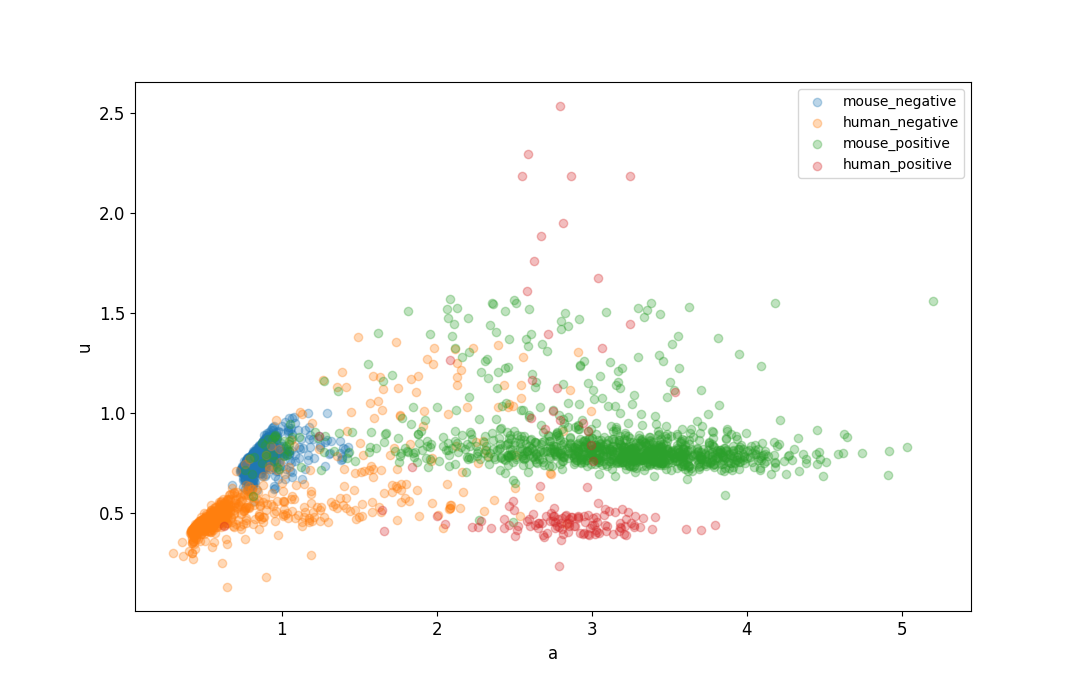
\includegraphics[width=\textwidth]{fig/all_cells}
	
	\caption{All data points from the four control data sets plotted along the axes activated value $a$ and unactivated values $u$.}
	\label{fig:all_cells}
\end{figure}

Differences in the axes $a$ and $u$ are present. On average the unactivated value $u$ and activated value $a$ are bigger in mouse t cells than the human counterparts. Looking at each of the parameters gathered from the approximation is possible by using the means and standard deviation of each parameter. These values are displayed in table~\ref{tab:mean_std_parameters}. It shows the mean $\mu$ and standard deviation $\sigma$ of the negative and positive control of mouse and human t cells.

\begin{table}[h!]
	\centering
	\begin{tabular}{|c|c|c|c|c|c|c|c|c|c|}
		\hline
		& & & $a$ & $u$ & $d$ & $k1$ & $k2$ & $w1$ & $w2$\\
		\hline
		\multirow{4}{*}{\rotatebox[origin=c]{90}{mouse}} & \multirow{2}{*}{\rotatebox[origin=c]{90}{pos}} & $\mu$ & 3.083 & 0.85 & 1.698 & 0.08 & -0.052 & 300.77 & 491.275\\
		\cline{3-10}
		& & $\sigma$ & 0.72 & 0.159 & 0.33 & 0.085 & 0.07 & 82.451 & 104.304\\
		\cline{2-10}
		& \multirow{2}{*}{\rotatebox[origin=c]{90}{neg}} & $\mu$ & 0.862 & 0.77 & 0.788 & 1.262 & -0.075 & 88.644 & 304.531\\
		\cline{3-10}
		& & $\sigma$ & 0.106 & 0.057 & 0.053 & 1.219 & 0.148 & 99.833 & 184.08\\
		\hline
		\multirow{4}{*}{\rotatebox[origin=c]{90}{human}} & \multirow{2}{*}{\rotatebox[origin=c]{90}{pos}} & $\mu$ & 2.854 & 0.553 &  1.916 & 0.23 & -0.033 & 113.595 & 438.763\\
		\cline{3-10}
		& & $\sigma$ & 0.357 & 0.294 & 0.44 & 0.219 & 0.073 & 59.7 & 175.998\\
		\cline{2-10}
		& \multirow{2}{*}{\rotatebox[origin=c]{90}{neg}} & $\mu$ & 0.864 & 0.543 & 0.604 & 0.58 & -0.19 & 169.394 & 528.006 \\
		\cline{3-10}
		& & $\sigma$ & 0.56 & 0.197 & 0.274 & 1.022 & 0.332 & 142.358 & 229.078 \\
		\hline
	\end{tabular}
	\caption{Mean $\mu$ and standard deviation $\sigma$ of the parameters of the approximation for positive and negative controls in human and mouse cells.}
	\label{tab:mean_std_parameters}
\end{table}

By comparing the means from table~\ref{tab:mean_std_parameters} we see that indeed the mean of $a$ and $u$ are higher or about equal in mouse cells. Differences in $d$, $k1$ and $k2$ are less pronounced and differ between positive and negative control. Differences in $w1$ and $w2$ are probably caused by differences in timing between the different recordings of the control groups. Therefore, comparing the means does not give much valuable information. In conclusion the differences are biggest in the parameter $u$.

\newpage
\section{Oscillation in Decrease}
\label{sec:oscillation_in_decrease}

Looking at the frequencies, amplitudes and phases returned from the approximation described in section~\ref{sec:adding_oscillation_to_the_approximation} gives us an idea with which period the typical t cell oscillates in \Calcium concentration during the decrease after activation. The figure~\ref{fig:freq_amp} shows violin plots of all three parameters in the positive control on human t cells. The means in this data set are 0.005 for the frequency, 0.01 for the amplitude and -0.001 for the phase. The details of the density distribution are shown in the width of each of the violin plots.

As some t cells do not oscillate, the approximation sometimes returns a misleading frequency with a low amplitude. We want to filter these cells before looking at the typical period with which the \Calcium concentration oscillates. We choose arbitrary threshold values, that seemed sensible to the author. Namely, all particles with an amplitude less than 0.1 or a frequency less than 0.005 are removed before once again looking at the average values. Now the average frequency is 0.008 with an average amplitude of 0.223. This corresponds to a period of oscillation being $1/freq = $ 125 seconds. Indeed, looking at the example provided in figure~\ref{fig:freq_amp}, this seems like a good estimate.

Lastly we compare this to the positive control in mouse cells. Before filtering the averages are 0.007 for the frequency, 0.071 for the amplitude and 0.288 for the phase. After filtering, with the same thresholds as for human cells, we have an average of 0.007 for the frequency and 0.177 for the amplitude. Converting this to the period gives us 143 seconds. This compares to the average period found in human t cells.

\begin{figure}[h!]
	\centering
	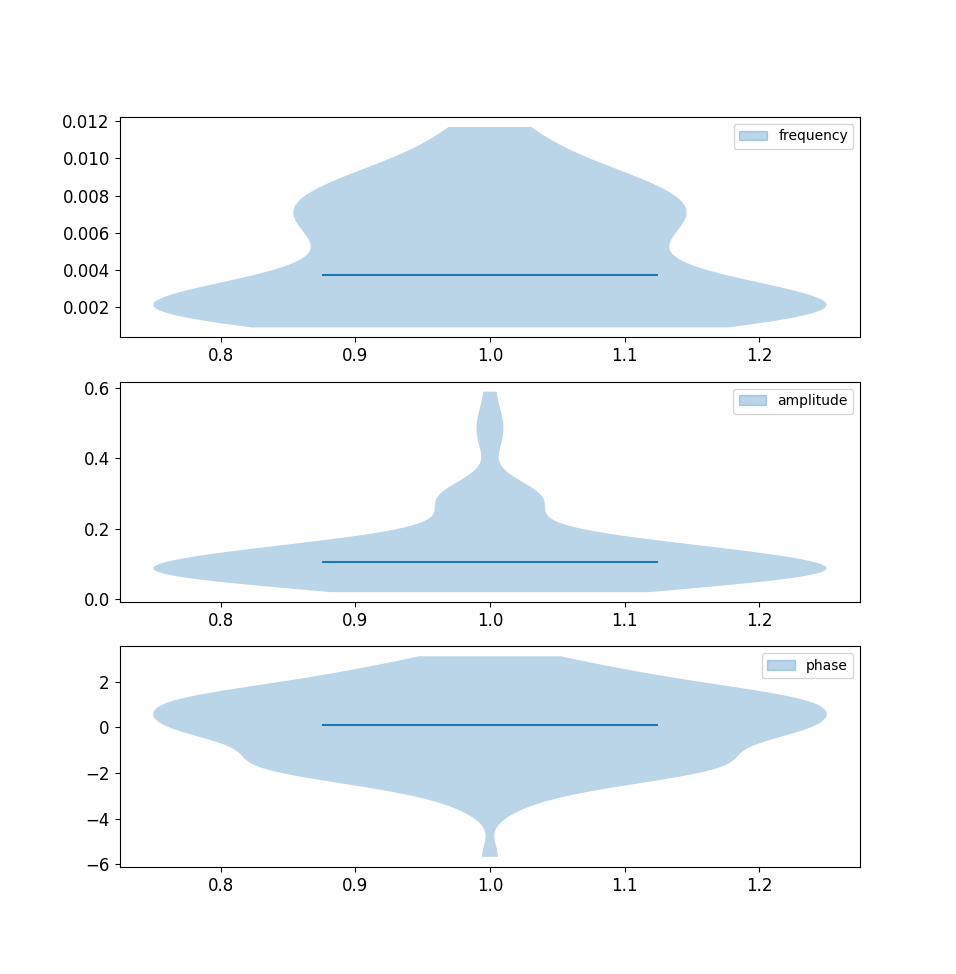
\includegraphics[width=0.9\textwidth]{fig/freq_amp}
	
	\caption{Violin plots of the frequencies, amplitudes and phases of the oscillation approximation in the positive control dataset of human t cells.}
	\label{fig:freq_amp}
\end{figure}

\newpage
\section{Types of Activated Cells}

It is interesting to see whether there are different types of activated cells. We find an answer by looking at the activated cells only. We have two data sets of activated cells, one from mouse cells and one from human cells. Naturally there will be differences between the two. This was further explored in section~\ref{sec:differences_between_mouse_and_human_cells}. By looking at only one data set of the positive control at a time we generate the images seen in figure~\ref{fig:positive_control}. To reduce the dimensionality once again Principal Component Analysis is used.

From figure~\ref{fig:positive_control}, it is not apparent that there are different types of activated cells.

Lastly we can have a look whether particles differ in the oscillation. Using the approximation of the oscillation and the filtering done in section~\ref{sec:oscillation_in_decrease} we can for example differ between oscillating t cells, marked by high amplitude and period around the expected 125 seconds, and non-oscillating t cells, marked by low amplitude or different period.

We note that out of 139 particles in the positive control of human t cells only 14 have the behaviour of a heavily oscillating t cell. In the mouse positive control it is 192 out of 1058.

\begin{figure}[h]
	\centering
	\begin{subfigure}{0.49\linewidth}
		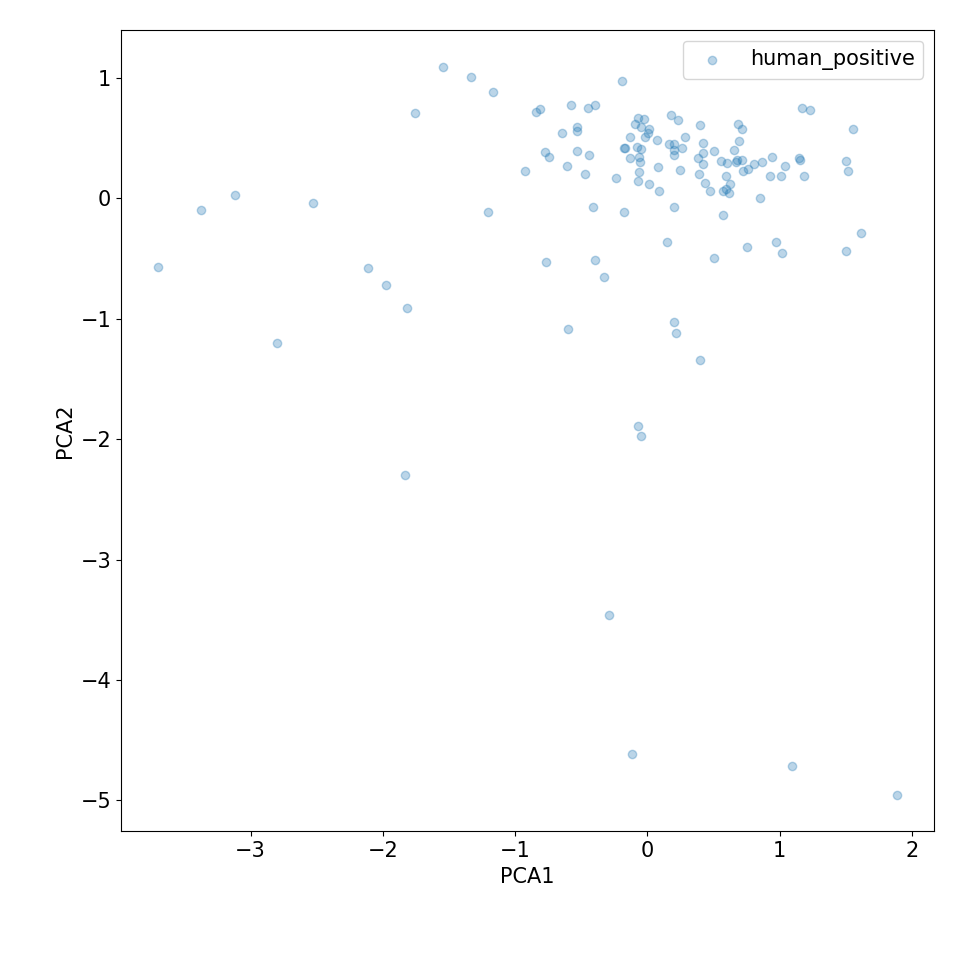
\includegraphics[width=\textwidth]{fig/positive_control_human}
	\end{subfigure}
	\hfill
	\begin{subfigure}{0.49\linewidth}
		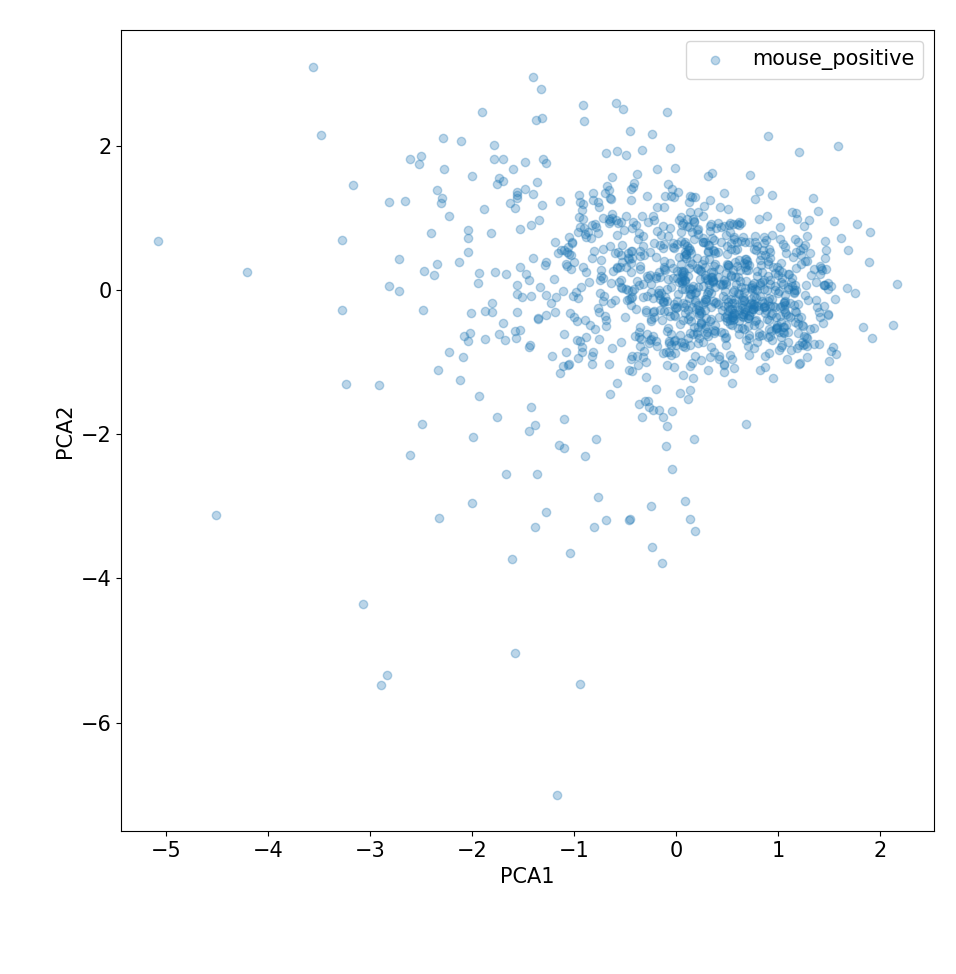
\includegraphics[width=\textwidth]{fig/positive_control_mouse}
	\end{subfigure}
	
	\caption{First two axes of the Principal Component Analysis of activated human and mouse t cells. There appear not be any major differences between the two types of t cells.}
	\label{fig:positive_control}
\end{figure}
\chapter{Discussion}
\label{chapter:conclusion}

This chapter gives answers to the questions from chapter~\ref{chapter:introduction} using the results from chapter~\ref{chapter:results} and gives an outlook which aspects could be improved in further work.

\begin{itemize}
	\item Which criteria can distinguish between unactivated, activated and pre-activated cells?
	
	Pre-activated cells can be detected by having a parameter $u$ that is bigger than ${\mu + 0.5 \sigma}$, with $\mu$ being the mean and $\sigma$ being the standard deviation of $u$. Distinguishing between activated and unactivated T cells can be done by the algorithm proposed in section~\ref{sec:proposed-algorithm}.
	\item Do different types of activated cells exists? How are they different?
	
	There are no apparent differences between different activated T cells. The parameters found behave according to a normal distribution. Differences can be found in how pronounced the oscillations are.
	\item With which frequencies does the Calcium concentration repeat after activation?
	
	The oscillations appear to have a frequency of about 0.0075 which corresponds to a period of 133 seconds in both human and mouse T cells.
	\item Is there a difference between mouse and human cells?
	
	There are differences between the two different types of T cells. The biggest differences are present in the parameter $u$ of the \Calcium concentration before activation.
\end{itemize}

As the first question is the most relevant we want to discuss the answer further. To give a value for accuracy achieved by the proposed algorithm we have to know how many T cells from the experiment dataset are activated. We do this by using some of the particles from the positive and negative control. Using random sampling we select some particles from each control data set to be the experiment data. Of course, we then have to remove these particles from the control data to avoid training on the data we test with. By varying the number of particles chosen from the two control data sets we can vary the percentage of activated cells in this generated experiment data. The results from this test can be found in table~\ref{tab:accuracy}.

\begin{table}[h]
	\centering
	\begin{tabular}{|c|c|c|}
		\hline
		\textbf{percentage activated} & \textbf{k-means output} & \textbf{gaussian mixture output}\\
		\hline
		\hline
		0\% & 5.5\% & 4\%\\
		\hline
		25\% & 27.5\% & 26\%\\
		\hline
		50\% & 49.5\% & 49.5\%\\
		\hline
		75\% & 72\% & 70.5\%\\
		\hline
		100\% & 96\% & 97.5\%\\
		\hline
	\end{tabular}
	\caption{Percentage activated output by k-means and gaussian Mixture for different true values of percentages of activated T cells.}
	\label{tab:accuracy}
\end{table}

We now discuss possible improvements. The proposed algorithm and subsequent analysis of the clustering performed can be improved by applying the discussed algorithm to enough data points to achieve a good approximation for average and standard deviation that hold for arbitrary data points from the same T cell line.

Another improvement can be made in the frequency analysis. Exploring what causes these oscillations can give a better understanding as to what type of oscillation is to be expected and how these might differ between different T cells. The assumption made in this work, that the oscillations can be modelled by a single sine wave, might prove wrong. In this case a different modelling approach has to be chosen. Alternatively, the output of the FFT can be used directly.

Lastly, the performance of the Python implementation given in the appendix~\ref{chapter:python_implementation} is suboptimal. Changing to other programming languages or improving the performance of the code in Python desirable.

\vspace{0.5cm}
\noindent
In summary this work proposed an algorithm for detecting activated T cells in \Calcium concentration recordings, without a need for user specified criteria for activation detection. The accuracy of this algorithm is acceptable, and the implementation is given in Python.


\printbibliography
\end{document}
